%\noindent
\justifying
\setlength{\parskip}{1em}

In this chapter, the experiments conducted in this thesis are described along with evaluation metrics and results. In Section \ref{EvaluationMetrics} the evaluation metrics like accuracy, precision, recall, confusion matrix, and F1-score are explained. These metrics are used to evaluate the domain gap between the distributions and quality of \ac{CycleGAN} generated document images. In section \ref{experiments} all the experiments that are conducted in this thesis are explained along with training plots, confusion matrices, and classification reports. Finally, in section \ref{results}, quantitative and qualitative results are discussed thoroughly.

\section{Evaluation Metrics}\label{EvaluationMetrics}

%\subsection{Accuracy}
%\subsection{Precision and Recall}
%\subsection{F1-score}

In machine learning research, numerous performance metrics have been introduced for neural networks. Each of which evaluates different aspects of neural network's performance. Hence, we need a specific set of performance metrics for a particular problem solved using neural networks. It's important to evaluate the performance of the neural network after training, using testing data, to determine its actual performance or generalization error on unseen data. In our thesis, we need to determine the performance of classifiers trained upon different data distributions using annotated real document images (test dataset). The popular classifier performance evaluation metrics are accuracy, precision, recall, confusion matrix, and F1-score \cite{powers2020evaluation}. The testing dataset used to evaluate the classifiers is unbalanced, hence metrics like weighted average and macro average F1-scores are essential for the performance comparison of the classifiers trained on different data distributions. 

The accuracy is the most common metric used to evaluate classifiers. It is the ratio of accurately classified data items to the total number of observations (equation \ref{accuracy}). The precision is ``how many selected items are relevant". ``To put it another way, out of the observations that an algorithm has predicted to be positive, how many of them are actually positive" \cite{vakili2020performance}. The precision is the ratio of the number of true positives divided by the sum of the true positive and false positives (equations \ref{precision}). The recall is ``how many relevant items are selected". ``In fact, out of the observations that are actually positive, how many of them have been predicted by the algorithm" \cite{vakili2020performance}. The recall is the ratio of the number of true positives divided by the sum of true positives and false negatives. In below equations \ref{accuracy}, \ref{precision}, and \ref{recall} the $TP$ means true positives, $TN$ means true negatives, $FP$ means false positives, and $FN$ means false negatives.



\begin{equation}\label{recall}
\textit{Recall} = \frac{TP}{TP + FN}
\end{equation}

\begin{equation}\label{precision}
\textit{Precision} = \frac{TP}{TP + FP}
\end{equation}


\begin{equation}\label{accuracy}
\textit{Accuracy} = \frac{TP + TN}{TP +TN+ FP + FN}
\end{equation}

F1-score is the harmonic mean of the precision and recall (equation \ref{f1-score}). The weighted average F1-score is determined by first calculating the F1-score of each class separately and each multiplied by the weight (the number of true instances for each class) and finally added together, hence favoring the majority class. The equation \ref{Weightedf1-score} represents the weighted average F1-score. The macro average F1-score computes the unweighted mean of separate F1-score of each class. The macro average F1-score does not take label inbalance into account. This leads to bigger penalization when the classifier does not perform well on minority classes. The equation \ref{macrof1-score} represents the macro average F1-score. In equations \ref{Weightedf1-score} and \ref{macrof1-score}, $N$ represents number of classes.

More information about accuracy, precision, recall, and F1-score can be found \href{https://en.wikipedia.org/wiki/Precision_and_recall}{here\footnotemark.}
\footnotetext{\url{https://en.wikipedia.org/wiki/Precision_and_recall} last access: 03.08.2021}


\begin{equation}\label{f1-score}
\textit{F1-score} = \frac{2 \times precision \times recall}{precision + recall}
\end{equation}


\begin{equation}\label{macrof1-score} 
\textit{Macro average F1-score} =  \frac{F1_{class1} + F1_{class2}+ ... + F1_{classN}}{N}
\end{equation}


\begin{equation}\label{Weightedf1-score} 
\textit{Weighted average F1-score} =  \frac{F1_{class1} \times W_1 + F1_{class2} \times W_2 + ... + F1_{classN} \times W_N}{N}
\end{equation}



The confusion matrix is the most intuitive metric to determine the accuracy of the classifiers. It is useful when the classifier has to classify more than two classes. A confusion matrix is a table that describes how well a classifier performs on a test dataset that is labeled or annotated. The instances of the true class are represented at each row of the confusion matrix whereas the instances of predicted class probabilities are represented by each column or vice versa. In our thesis confusion matrix is extensively used to analyze the performance of the classifiers trained on different data distributions. More information about the confusion matrix can be found \href{https://en.wikipedia.org/wiki/Confusion_matrix}{here}\footnotemark.
\footnotetext{\url{https://en.wikipedia.org/wiki/Confusion_matrix} last access: 03.08.2021}


\section{Experiments}\label{experiments}


In this thesis, several experiments were performed to understand the domain gap between data distributions. Three data distributions are considered for the experiments. Each data distribution represents a different domain. The synthetic document images represent the synthetic data distribution. The faxified document images represent faxified data distribution. The \ac{CycleGAN} generated images represent \ac{CycleGAN} generated data distribution. The goal of the experiments is to illustrate and analyze the domain gap between the real data distribution and above mentioned three data distributions. Also, one of the experiments was performed to determine the quality of \ac{CycleGAN} generated document images compared to the real document images. Now let's begin with the description of the experiments. First, the classifier(table \ref{table:ClassifierArchitecture}) is trained on synthetic document images and its performance is evaluated on annotated real document images. Second, the new classifier with the same architecture is trained on faxified document images and its performance is evaluated on annotated real document images. Third, the \ac{CycleGAN} is trained using synthetic document images and real document images and at the end of every epoch, the checkpoint is saved. As mentioned in training details \ref{TrainingDetailsCycleGAN}, \ac{CycleGAN} is trained for 20 epochs. 

Once training is finished, the latest saved checkpoint can be loaded to generate or transform images. The \ac{CycleGAN} trained considering synthetic data distribution as a source domain and real data distribution as a target domain. This means the synthetic document images represent the source domain and real document images represent the target domain. Next, the latest checkpoint is loaded, as we only need a generator $G$ to transform images from the source domain to the target domain. Hence, generator $G$ is retrieved to transform 100,000 synthetic document images into 100,000 realistic document images. We call these realistic document images as \ac{CycleGAN} generated document images which represents \ac{CycleGAN} generated data distribution. Further, 100,000 \ac{CycleGAN} generated document images are used to train another new classifier with the same architecture as the previous, and its performance is evaluated on annotated real document images. The experiment aims to understand the quality of the images generated by \ac{CycleGAN}. Especially, how efficiently \ac{CycleGAN} was able to close the domain gap between synthetic data distribution and real data distribution by generating quality images using generator $G$ in \ac{CycleGAN}. The evaluation metrics like accuracy, weighted average F1-score, and macro average F1-score \cite{lipton2014thresholding} are used to understand the contrast between the performance of the classifiers using annotated real document images.

\subsection{Experiment Steps}


\begin{enumerate}
    \itemsep0em 
    \item Train a classifier on synthetic document images and evaluate its classification performance on the annotated real document images.
    \item Train a classifier on faxified document images and evaluate its classification performance on the annotated real document images.
    \item Train a \ac{CycleGAN} using synthetic document images and real document images.
    \item Generate realistic document images using generator $G$ from the trained \ac{CycleGAN} model. As mentioned above realistic document images are also called \ac{CycleGAN} generated document images.
    \item Train a classifier on \ac{CycleGAN} generated document images and evaluate its classification performance on the annotated real document images.
    \item Compare the classification performance of the above three classifiers on the annotated real document images to illustrate the domain gap between real data distribution and other three distributions like synthetic data distribution, faxified data distribution, and \ac{CycleGAN} generated data distribution. The performance of a classifier trained upon \ac{CycleGAN} generated data distribution using annotated real document images describes, how close is the \ac{CycleGAN} generated data distribution to the real data distribution. Simply this approach determines the quality of the \ac{CycleGAN} generated document images compared to real document images.
\end{enumerate}


\subsection{\ac{CycleGAN} Training}

The \ac{CycleGAN} consists of two generators $G$ and $F$ and two discriminators $D_X$ and $D_Y$. Domain $X$ represents the source domain and domain $Y$ represents the target domain. The aim is to transform synthetic document images into realistic document images. Hence, the synthetic document images represent the source domain and real document images represent the target domain.

\begin{figure}[H]
  \centering
  \begin{minipage}[b]{0.49\textwidth}
    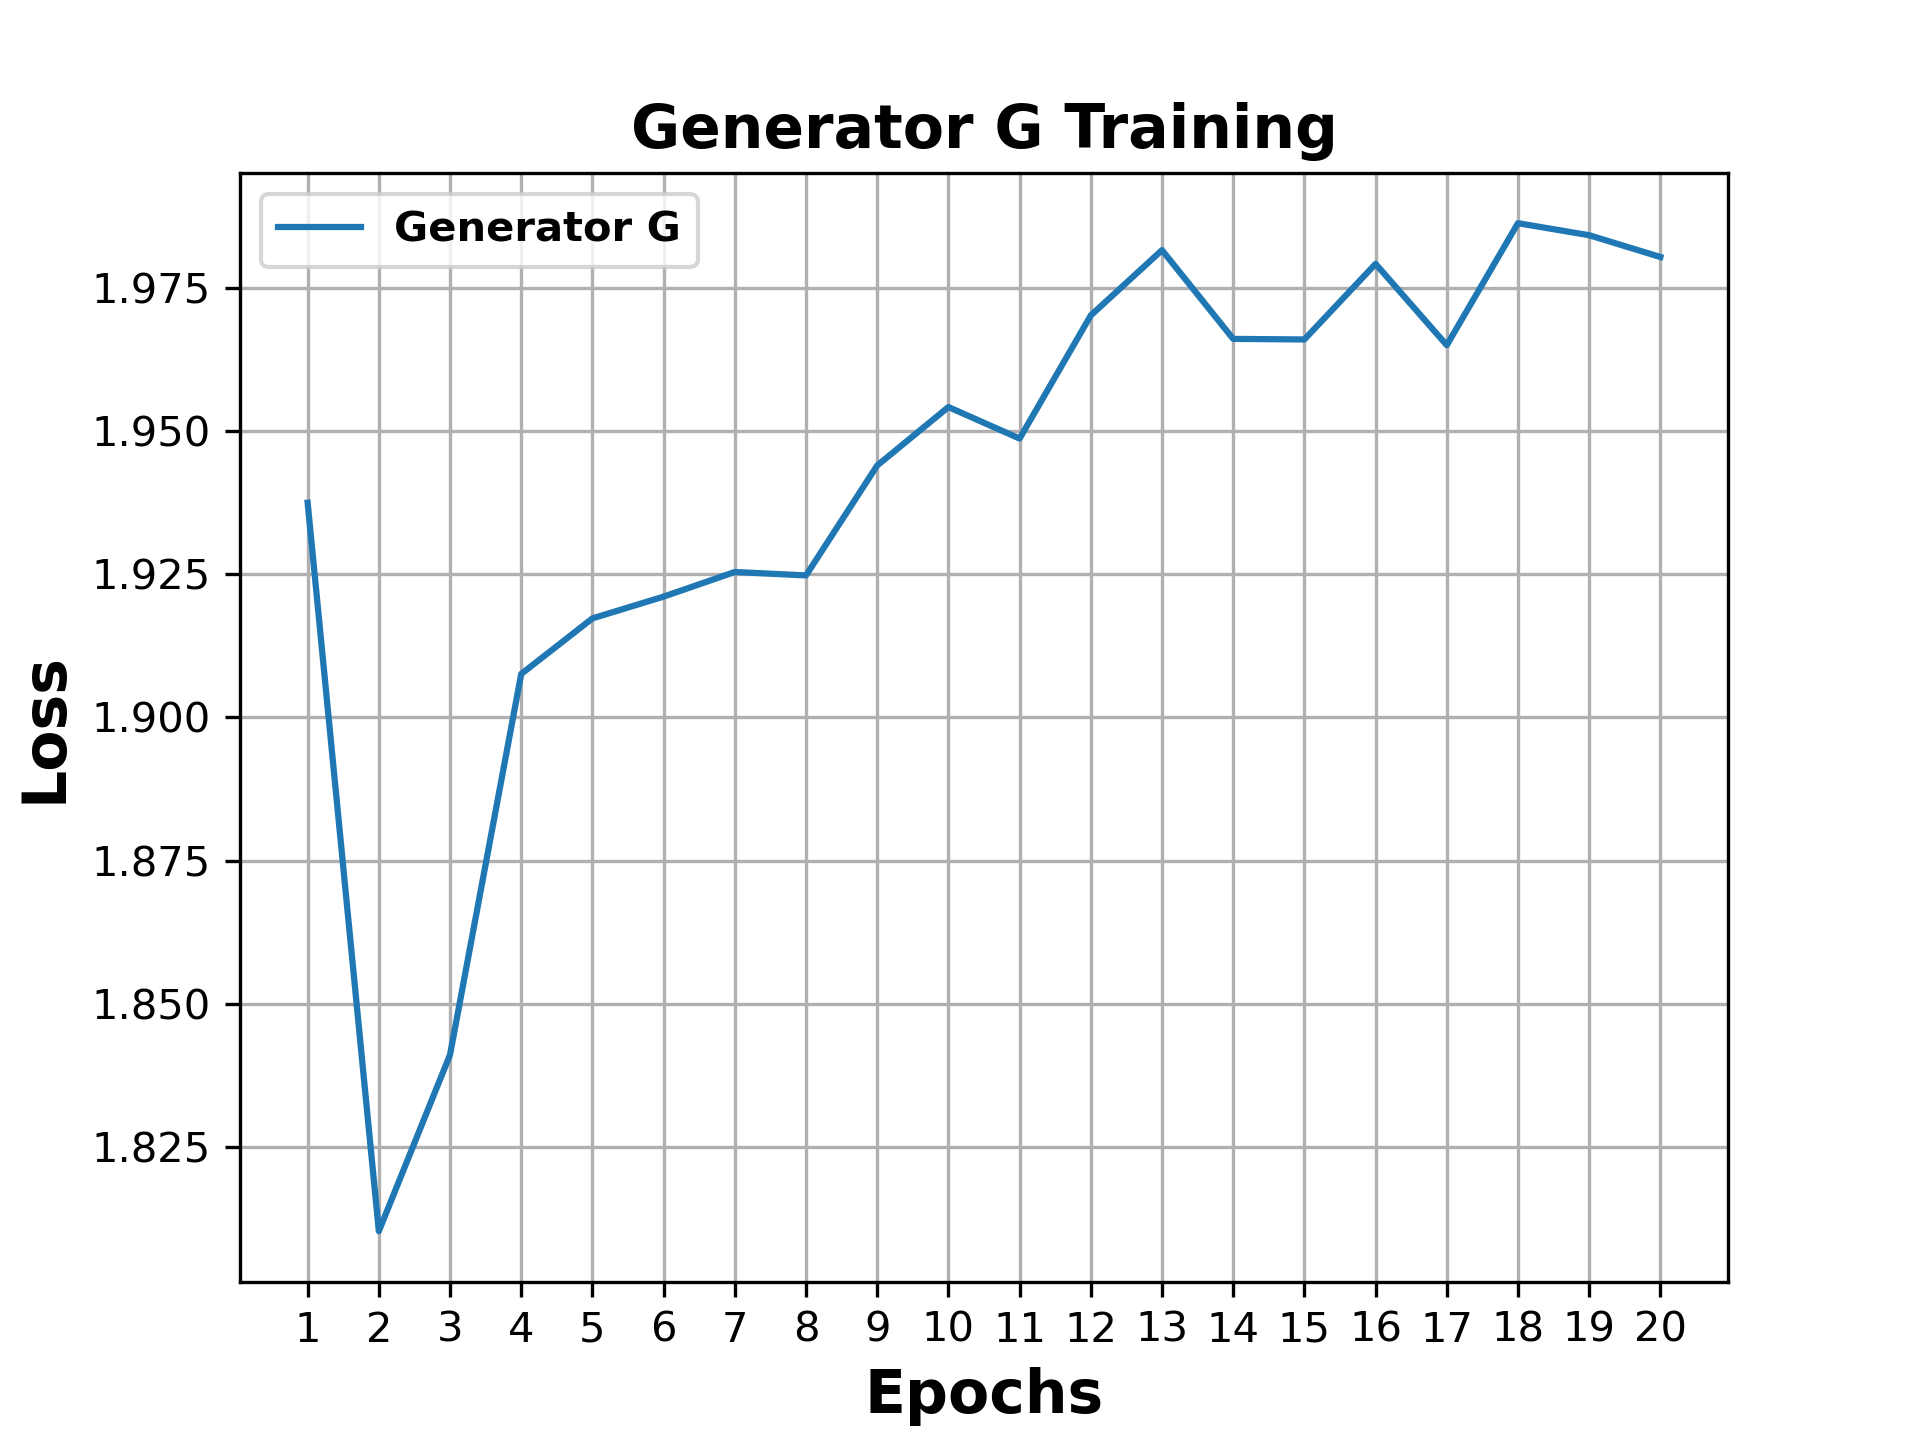
\includegraphics[width=\textwidth]{images/Evaluation/GeneratorGTraining.png}
    \caption[\ac{CycleGAN} generator $G$ training epochs vs loss plot.]{\ac{CycleGAN} generator $G$ training epochs vs loss plot.}
    \label{fig:generatorG}
  \end{minipage}
  \hfill
  \begin{minipage}[b]{0.49\textwidth}
    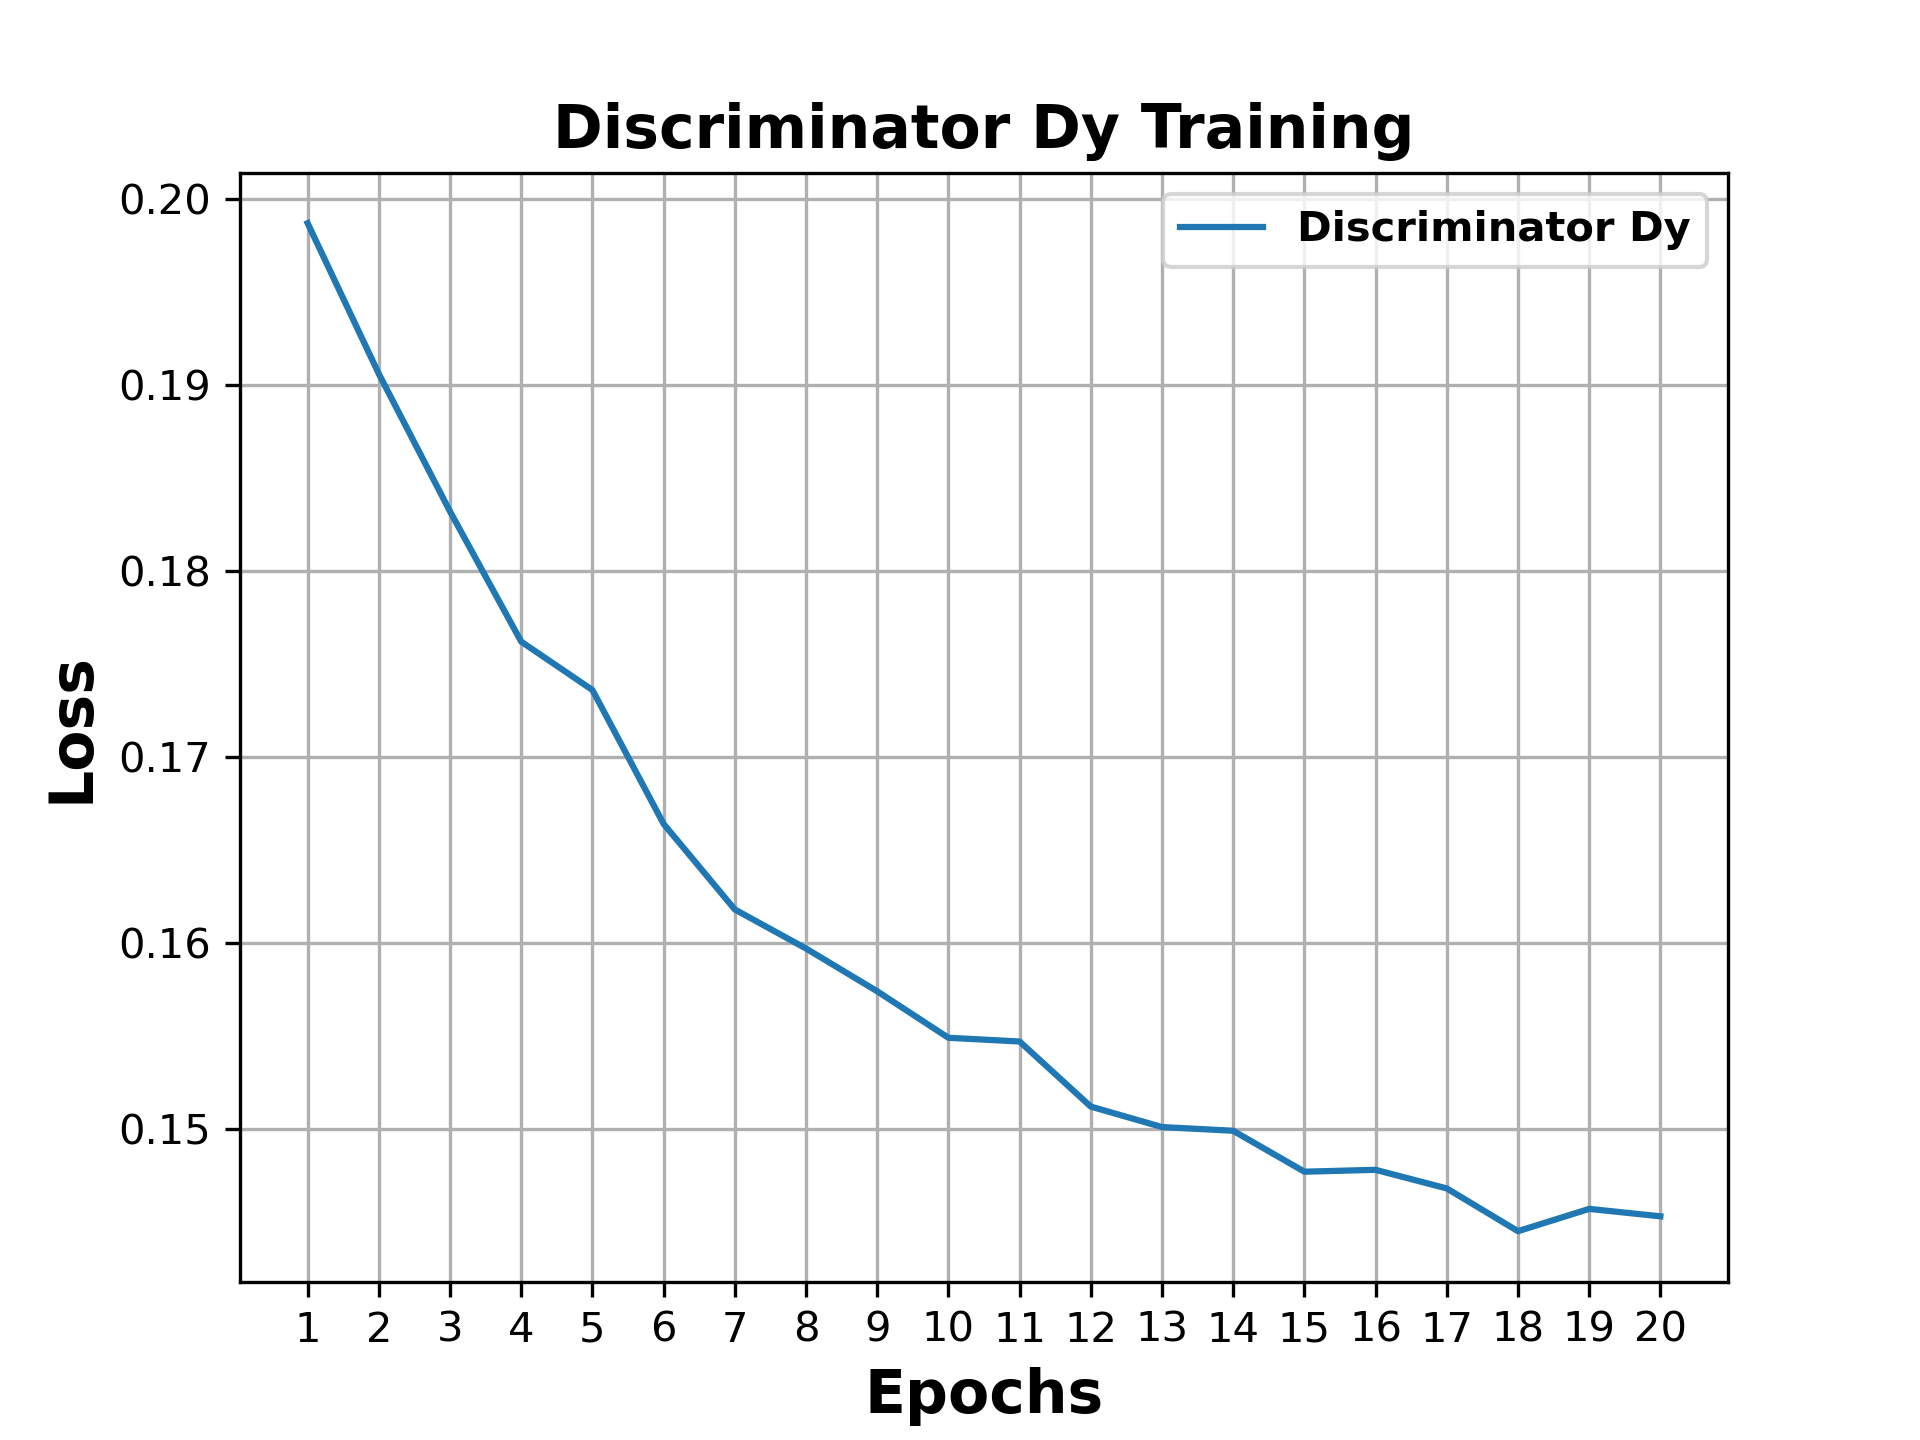
\includegraphics[width=\textwidth]{images/Evaluation/DiscriminatorDyTraining.png}
    \caption[\ac{CycleGAN} discriminator $D_Y$ training epochs vs loss plot.]{\ac{CycleGAN} discriminator $D_Y$ training epochs vs loss plot.}
    \label{fig:discriminatorDy}
  \end{minipage}
\end{figure}

\begin{figure}[H]
  \centering
  \begin{minipage}[b]{0.49\textwidth}
    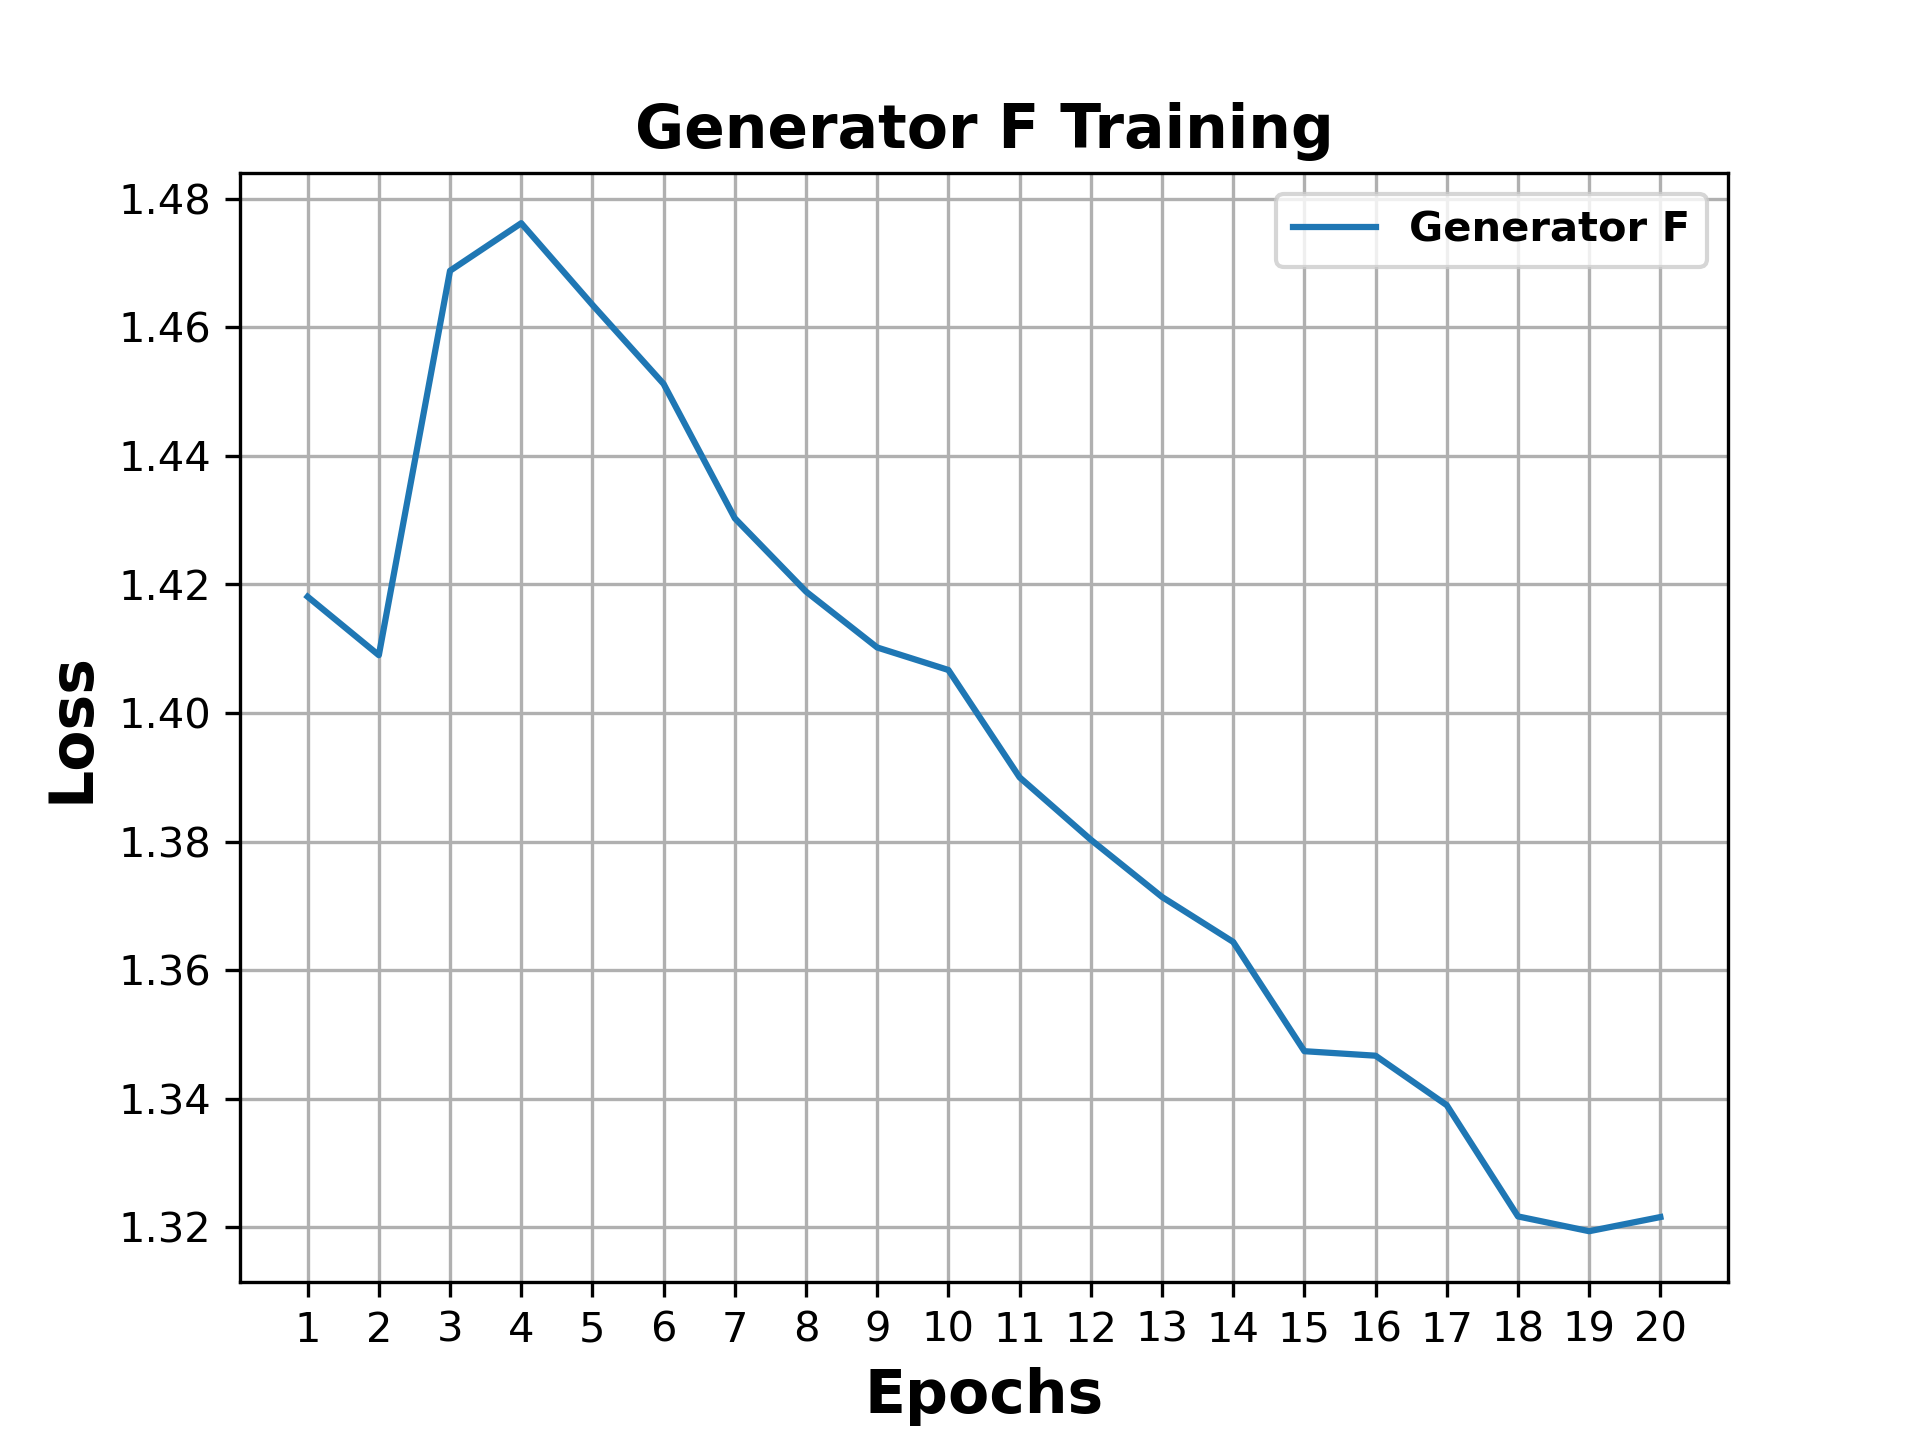
\includegraphics[width=\textwidth]{images/Evaluation/GeneratorFTraining.png}
    \caption[\ac{CycleGAN} generator $F$ training epochs vs loss plot.]{\ac{CycleGAN} generator $F$ training epochs vs loss plot.}
    \label{fig:generatorF}
  \end{minipage}
  \hfill
  \begin{minipage}[b]{0.49\textwidth}
    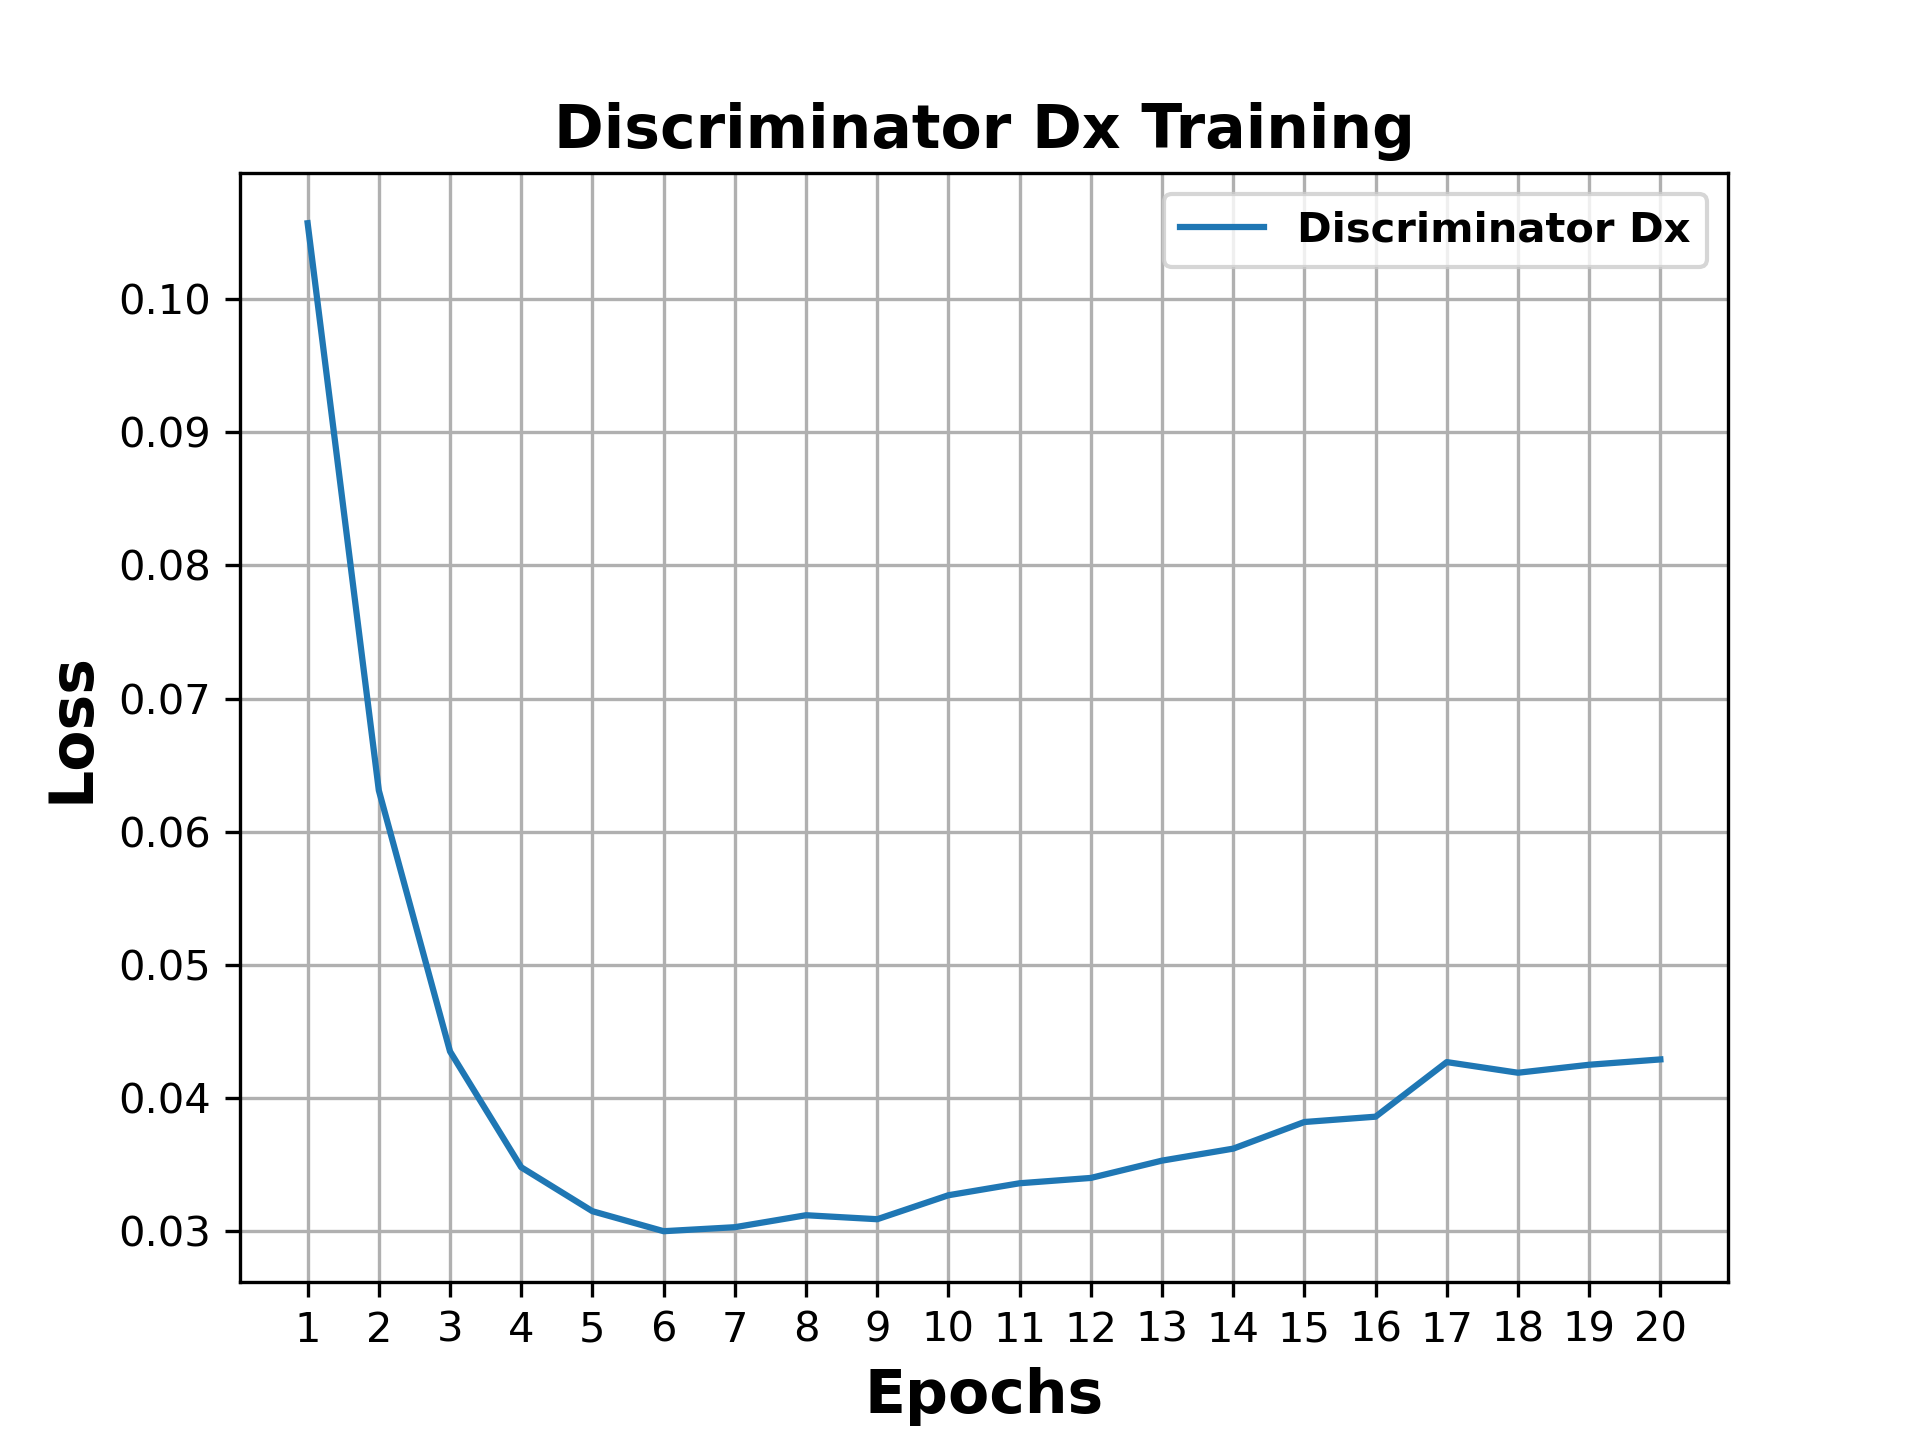
\includegraphics[width=\textwidth]{images/Evaluation/DiscriminatorDxTraining.png}
    \caption[\ac{CycleGAN} discriminator $D_X$ training epochs vs loss plot.]{\ac{CycleGAN} discriminator $D_X$ training epochs vs loss plot.}
    \label{fig:discriminatorDx}
  \end{minipage}
\end{figure}

The training plots of generators $G$ and $F$ are shown in figure \ref{fig:generatorG} and \ref{fig:generatorF} respectively. The training plots of discriminators $D_X$ and $D_Y$ are shown in figure \ref{fig:discriminatorDx} and \ref{fig:discriminatorDy} respectively. 


\subsection{Training a Classifier on Synthetic Document Images}\label{trainingsyntheticclassifier}





\begin{figure}[H]
  \centering
  \begin{minipage}[b]{0.49\textwidth}
    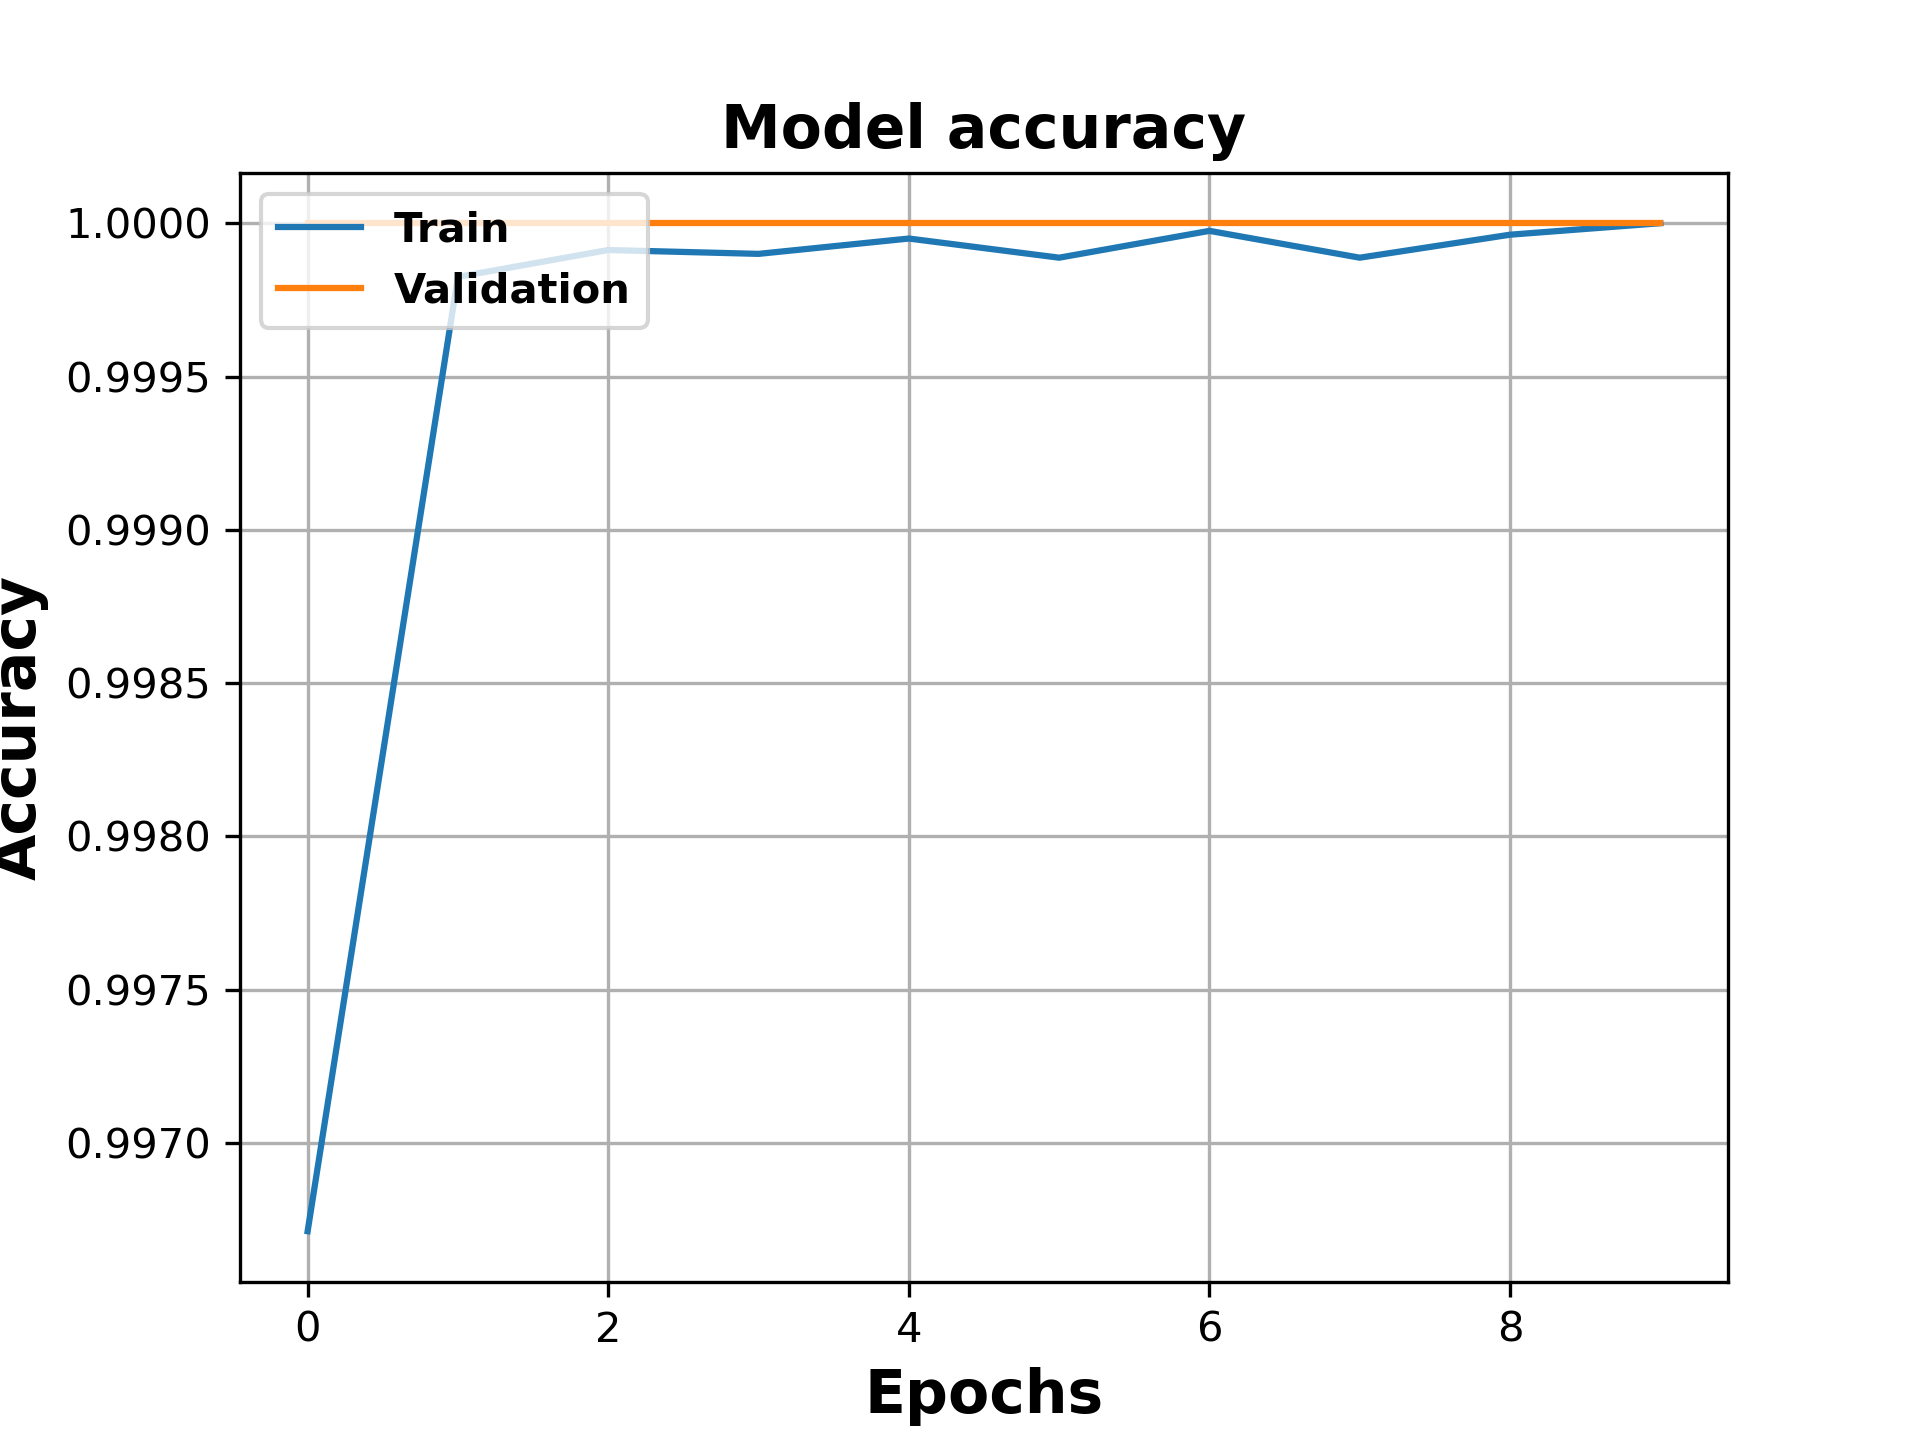
\includegraphics[width=\textwidth]{images/Evaluation/Synthetic_Data_Classifier_2021-05-31_16-40-33_Accuracy.png}
    \caption[Epochs vs accuracy plot while training a classifier on synthetic document images.]{Epochs vs accuracy plot while training a classifier on synthetic document images.}
    \label{fig:SyntheticClassifierAcc}
  \end{minipage}
  \hfill
  \begin{minipage}[b]{0.49\textwidth}
    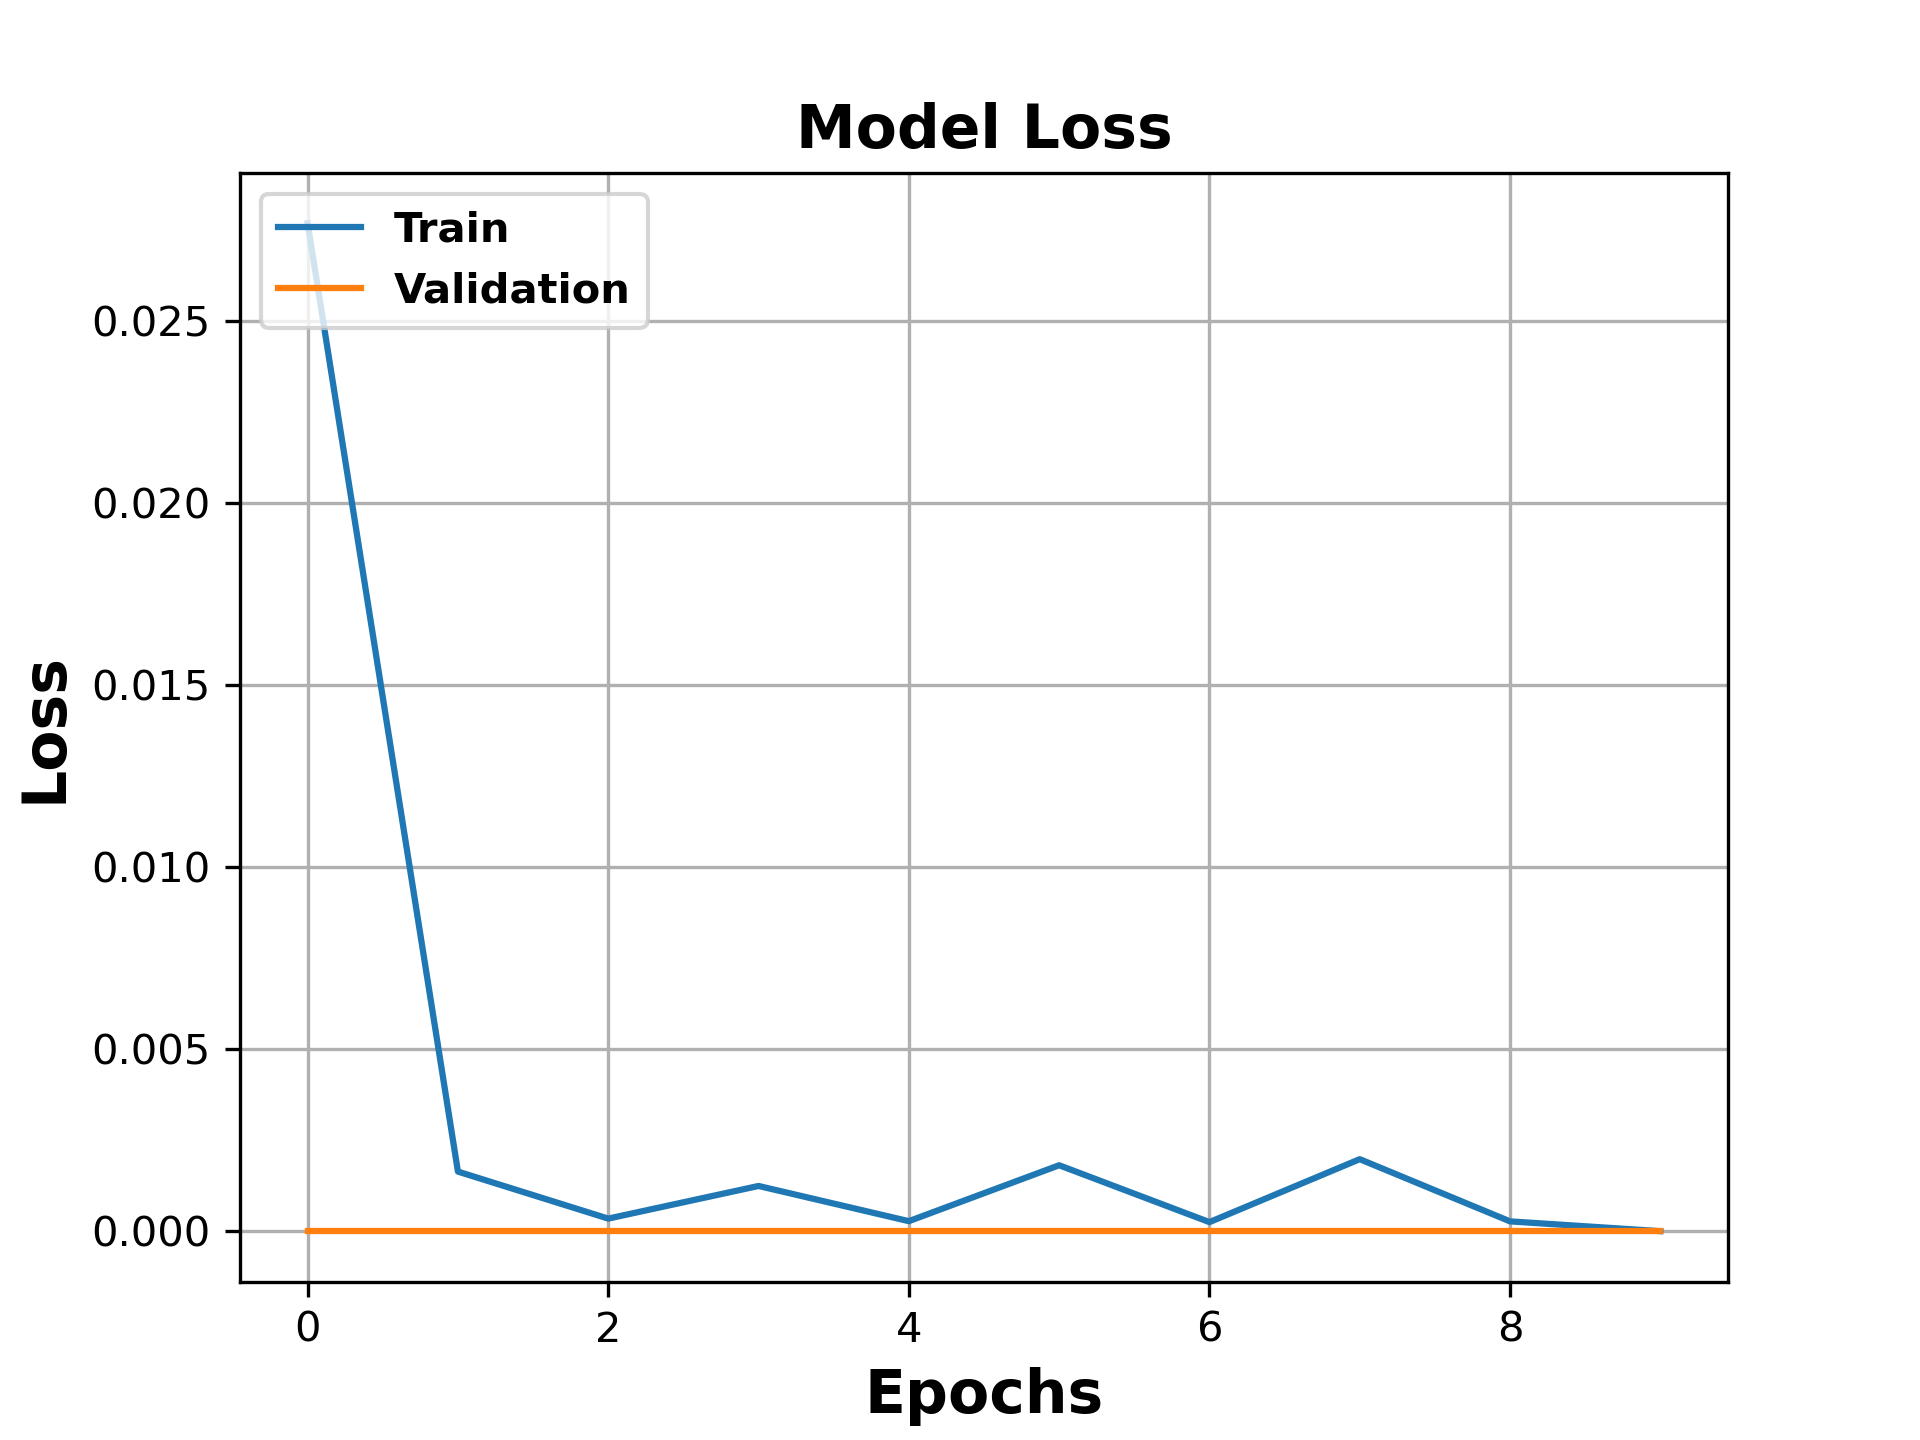
\includegraphics[width=\textwidth]{images/Evaluation/Synthetic_Data_Classifier_2021-05-31_16-40-33_Loss.png}
    \caption[Epochs vs loss plot while training a classifier on synthetic document images.]{Epochs vs loss plot while training a classifier on synthetic document images.}
    \label{fig:SyntheticClassifierLoss}
  \end{minipage}
\end{figure}


\begin{center}
\begin{table}[H]
    \centering
    \begin{center}
    \begin{tabular}{P{0.22\linewidth} P{0.10\linewidth} P{0.10\linewidth} P{0.10\linewidth} P{0.10\linewidth}} 
        \toprule
            & Precision & Recall & F1-score & Support\\[0.0ex] 
        \midrule
        DE\_LY\_Arm\_2020-01 & 0.65 & 0.50 & 0.56 & 44\\[0.0ex]
        \midrule
        DE\_LY\_Bein\_2018-08 & 0.50 & 0.02 & 0.04 & 47\\[0.0ex]
        \midrule
        DE\_LY\_Bein\_2019-01 & 0.06 & 0.90 & 0.11 & 50\\[0.0ex]
        \midrule
        DE\_LY\_Bein\_2019-07 & 0.36 & 0.20 & 0.26 & 60\\[0.0ex]
        \midrule
        DE\_LY\_Bein\_2020-01 & 0.96 & 0.21 & 0.34 & 624\\[0.0ex]
        \midrule
        DE\_LY\_Bein\_2020-03 & 0.24 & 0.25 & 0.24 & 128\\[0.0ex]
        \midrule
        DE\_LY\_Hand\_2020-01 & 0.70 & 0.44 & 0.54 & 16\\[0.0ex]
        \midrule
        DE\_PH\_Bein\_2018-09 & 0.10 & 0.14 & 0.12 & 22\\[0.0ex]
        \midrule
        DE\_PH\_Bein\_2019-02 & 0.12 & 0.04 & 0.06 & 28\\[0.0ex]
        \midrule
        DE\_PH\_Bein\_2020-01 & 0.95 & 0.51 & 0.26 & 143\\[0.0ex]
        \midrule
        \midrule
        Accuracy              &      &      & \bf{0.25} & 1162\\[0.0ex]
        Macro average             & 0.46 & 0.29 &  \bf{0.27} & 1162\\[0.0ex]
        Weighted average          & 0.74 & 0.25 &  \bf{0.31} & 1162\\[0.0ex]
        \bottomrule
    \end{tabular}
    \caption[Classification report generated after the classifier is trained on synthetic document images, its classification performance evaluated on the annotated real document images.]{Classification report generated after the classifier is trained on synthetic document images, its classification performance evaluated on the annotated real document images.}
    \label{table:SyntheticClassificationReport}
    \end{center}
\end{table}
\end{center}



\subsection{Training a Classifier on \ac{CycleGAN} Generated Document Images}




\begin{figure}[H]
  \centering
  \begin{minipage}[b]{0.45\textwidth}
    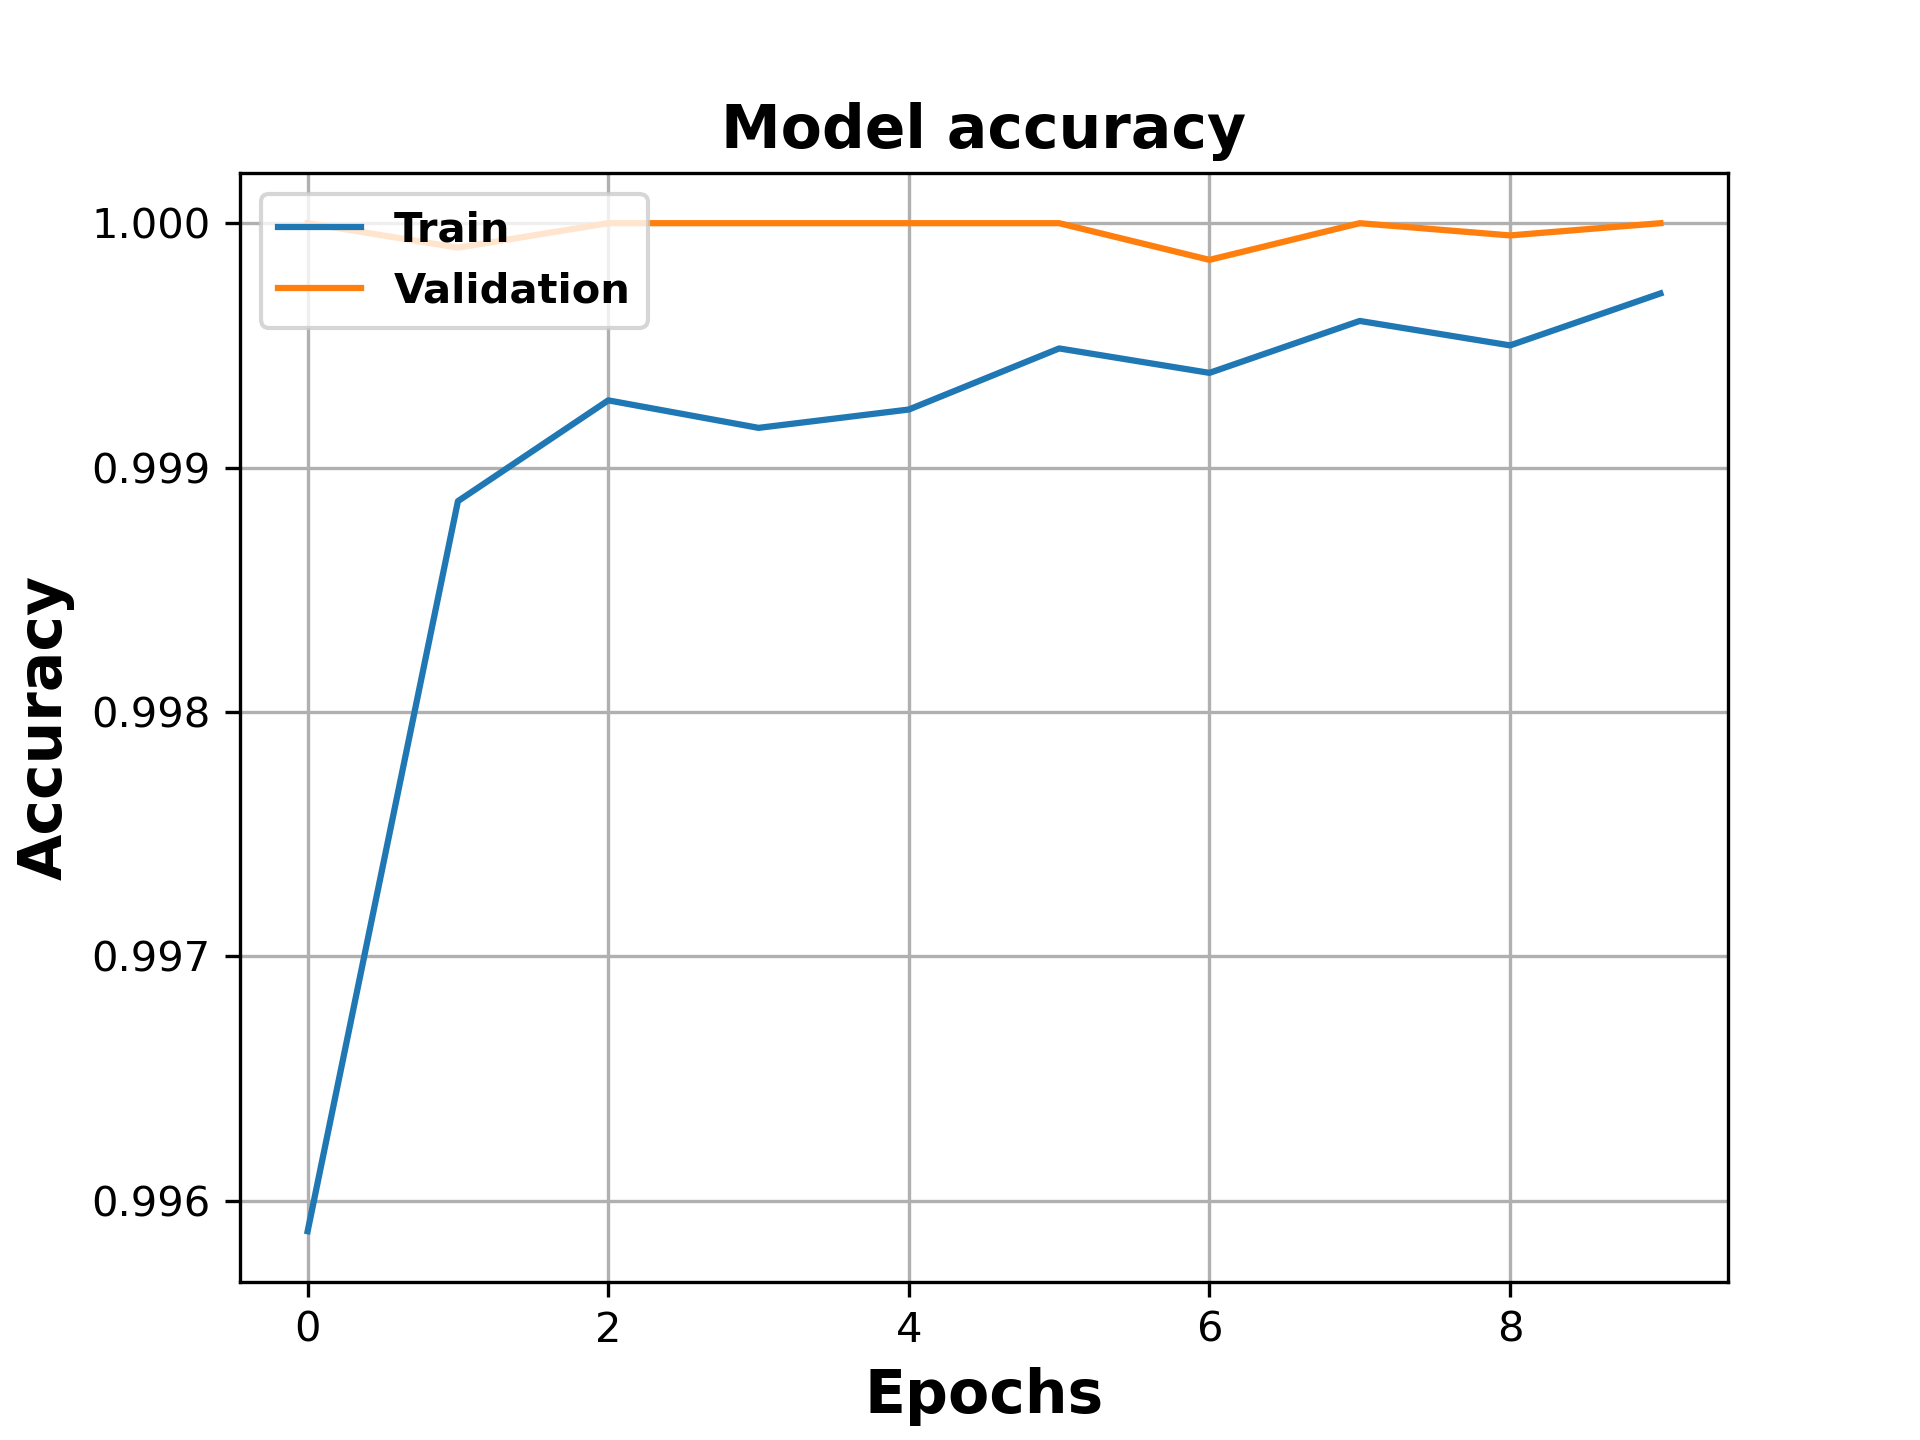
\includegraphics[width=\textwidth]{images/Evaluation/CycleGAN_Generated_Data_Classifier_2021-06-02_21-55-39_Accuracy.png}
    \caption[Epochs vs accuracy plot while training a classifier on \ac{CycleGAN} generated document images.]{Epochs vs accuracy plot while training a classifier  on \ac{CycleGAN} generated document images.}
    \label{fig:SyntheticClassifierAcc}
  \end{minipage}
  \hfill
  \begin{minipage}[b]{0.45\textwidth}
    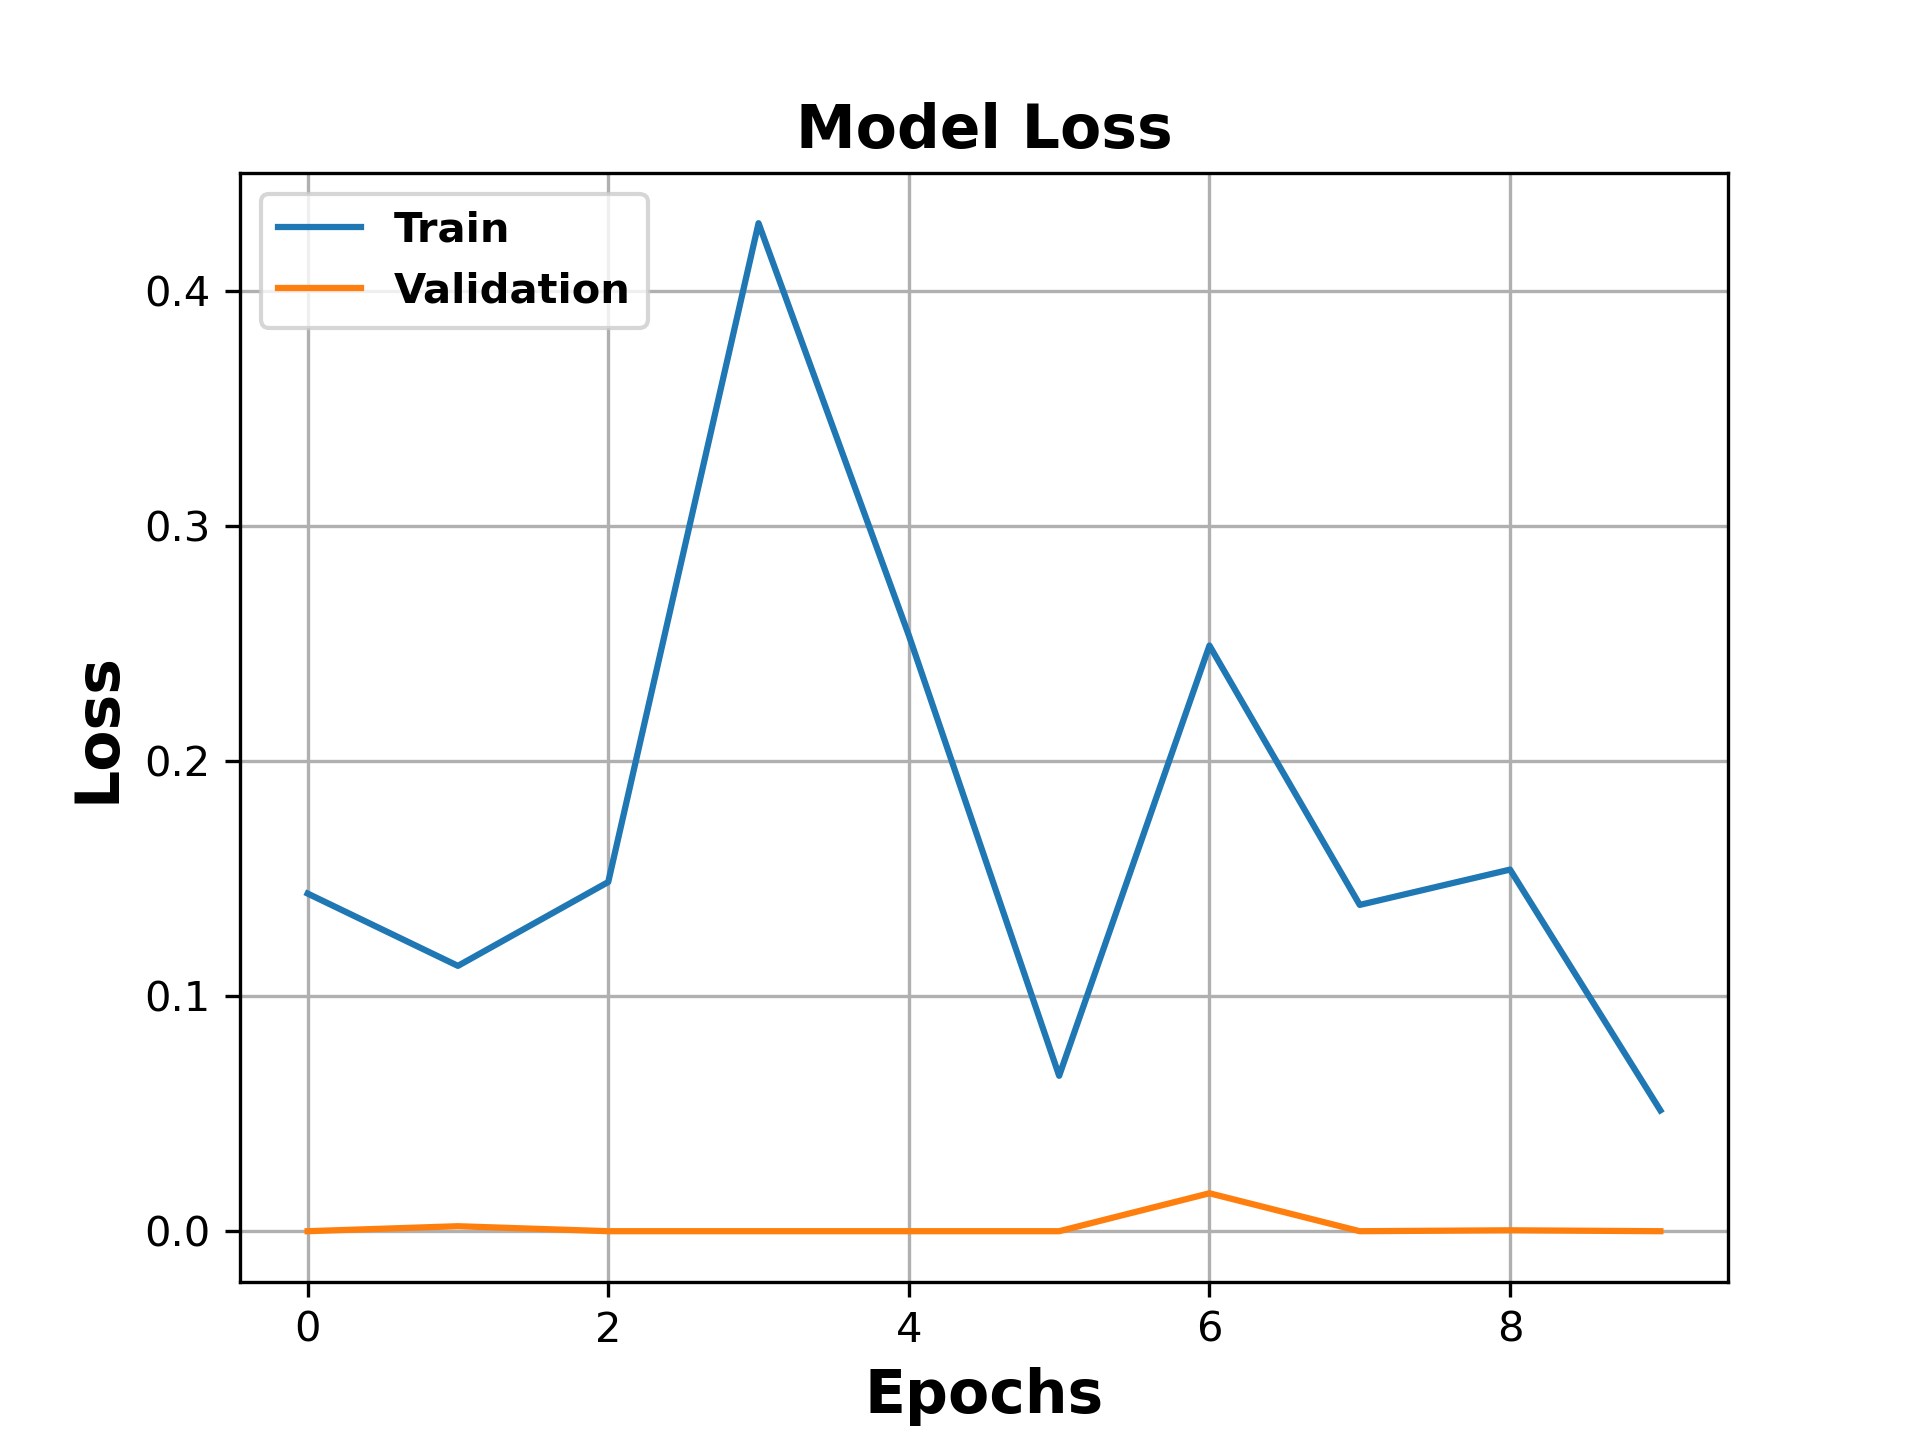
\includegraphics[width=\textwidth]{images/Evaluation/CycleGAN_Generated_Data_Classifier_2021-06-02_21-55-39_Loss.png}
    \caption[Epochs vs loss plot while training a classifier on \ac{CycleGAN} generated document images.]{Epochs vs loss plot while training a classifier on \ac{CycleGAN} generated document images.}
    \label{fig:SyntheticClassifierLoss}
  \end{minipage}
\end{figure}


\begin{center}
\begin{table}[H]
    \begin{center}
    \begin{tabular}{P{0.22\linewidth} P{0.10\linewidth} P{0.10\linewidth} P{0.10\linewidth} P{0.10\linewidth}} 
	        \toprule
            & Precision & Recall & F1-score & Support\\[0.0ex] 
        \midrule
        DE\_LY\_Arm\_2020-01 & 0.53 & 0.75 & 0.62 & 44\\[0.0ex]
        \midrule
        DE\_LY\_Bein\_2018-08 & 0.21 & 0.28 & 0.24 & 47\\[0.0ex]
        \midrule
        DE\_LY\_Bein\_2019-01 & 0.16 & 0.14 & 0.15 & 50\\[0.0ex]
        \midrule
        DE\_LY\_Bein\_2019-07 & 0.11 & 0.83 & 0.19 & 60\\[0.0ex]
        \midrule
        DE\_LY\_Bein\_2020-01 & 0.72 & 0.07 & 0.12 & 624\\[0.0ex]
        \midrule
        DE\_LY\_Bein\_2020-03 & 0.16 & 0.34 & 0.22 & 128\\[0.0ex]
        \midrule
        DE\_LY\_Hand\_2020-01 & 0.80 & 0.75 & 0.77 & 16\\[0.0ex]
        \midrule
        DE\_PH\_Bein\_2018-09 & 0.07 & 0.05 & 0.06 & 22\\[0.0ex]
        \midrule
        DE\_PH\_Bein\_2019-02 & 0.33 & 0.46 & 0.39 & 28\\[0.0ex]
        \midrule
        DE\_PH\_Bein\_2020-01 & 0.70 & 0.67 & 0.68 & 143\\[0.0ex]
        \midrule
        \midrule
        Accuracy              &      &      & \bf{0.27} & 1162\\[0.0ex]
        Macro average             & 0.38 & 0.43 &  \bf{0.34} & 1162\\[0.0ex]
        Weighted average          & 0.55 & 0.27 &  \bf{0.25} & 1162\\[0.0ex]
        \bottomrule
    \end{tabular}
    \caption[Classification report generated after the classifier is trained on synthetic document images, its classification performance evaluated on the annotated real document images.]{Classification report generated after the classifier is trained on synthetic document images, its classification performance evaluated on the annotated real document images.}
    \label{table:SyntheticClassificationReport}
    \end{center}
\end{table}
\end{center}










\subsection{Training a Classifier on Faxified Document Images}\label{trainingfaxifiedclassifier}

The faxification process mimics the way the fax machine works. Usually, fax machines transmit only black-and-white images, which might be dirty and are generally also not aligned perfectly. This leads to several common artifacts being introduced into transferred images, so faxification process attempts to mimic those introductions of artifacts into images. The faxification process transforms clean gray-scale synthetic document images in such a way like it was sent via fax. The faxification process is not deterministic, involves randomness during the process of faxification of the images. It uses several image transformations like gamma transformation, brightness transformation, 180-degree rotations, resizing, rescaling, binarization, adding noise, adding verticle lines, and conversion to a grayscale image. The faxification process can be visualized in figure \ref{fig:FaxificationProcess}. In figure \ref{fig:FaxificationProcessZoomed}, it is visible a snippet from the synthetic document image that has transformed randomly into different image transformations when it has been through the faxification process.



\begin{figure}[H]
  \centering
  \begin{minipage}[b]{0.49\textwidth}
    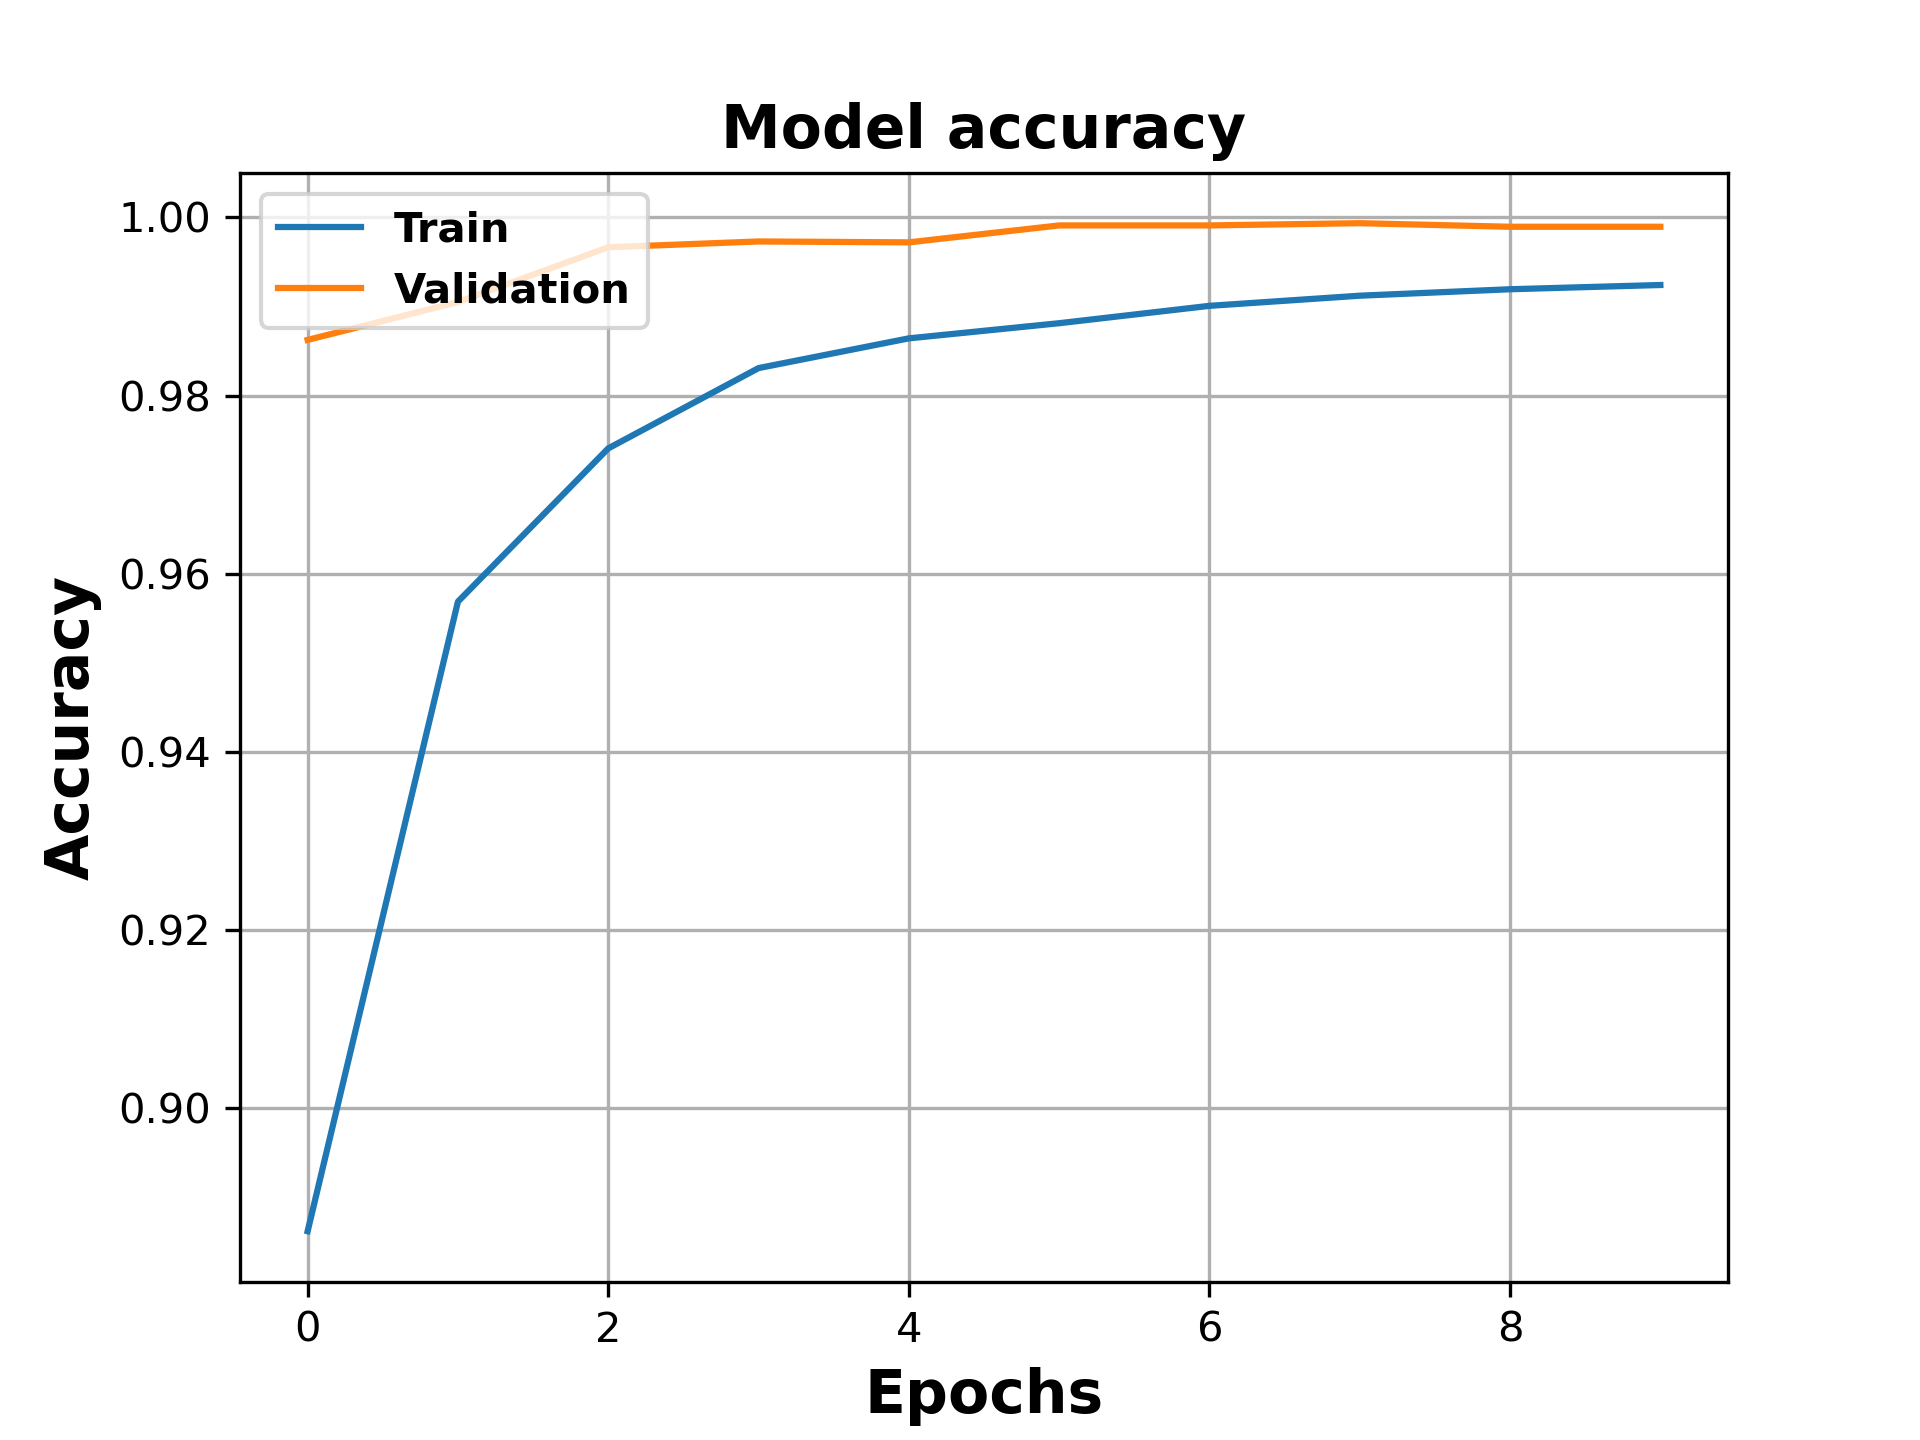
\includegraphics[width=\textwidth]{images/Evaluation/Faxified_Data_Classifier_2021-05-31_19-31-35_Accuracy.png}
    \caption[Epoch vs Accuracy Plot.]{Epoch vs Accuracy Plot.}
    \label{fig:FaxifiedClassifierAcc}
  \end{minipage}
  \hfill
  \begin{minipage}[b]{0.49\textwidth}
    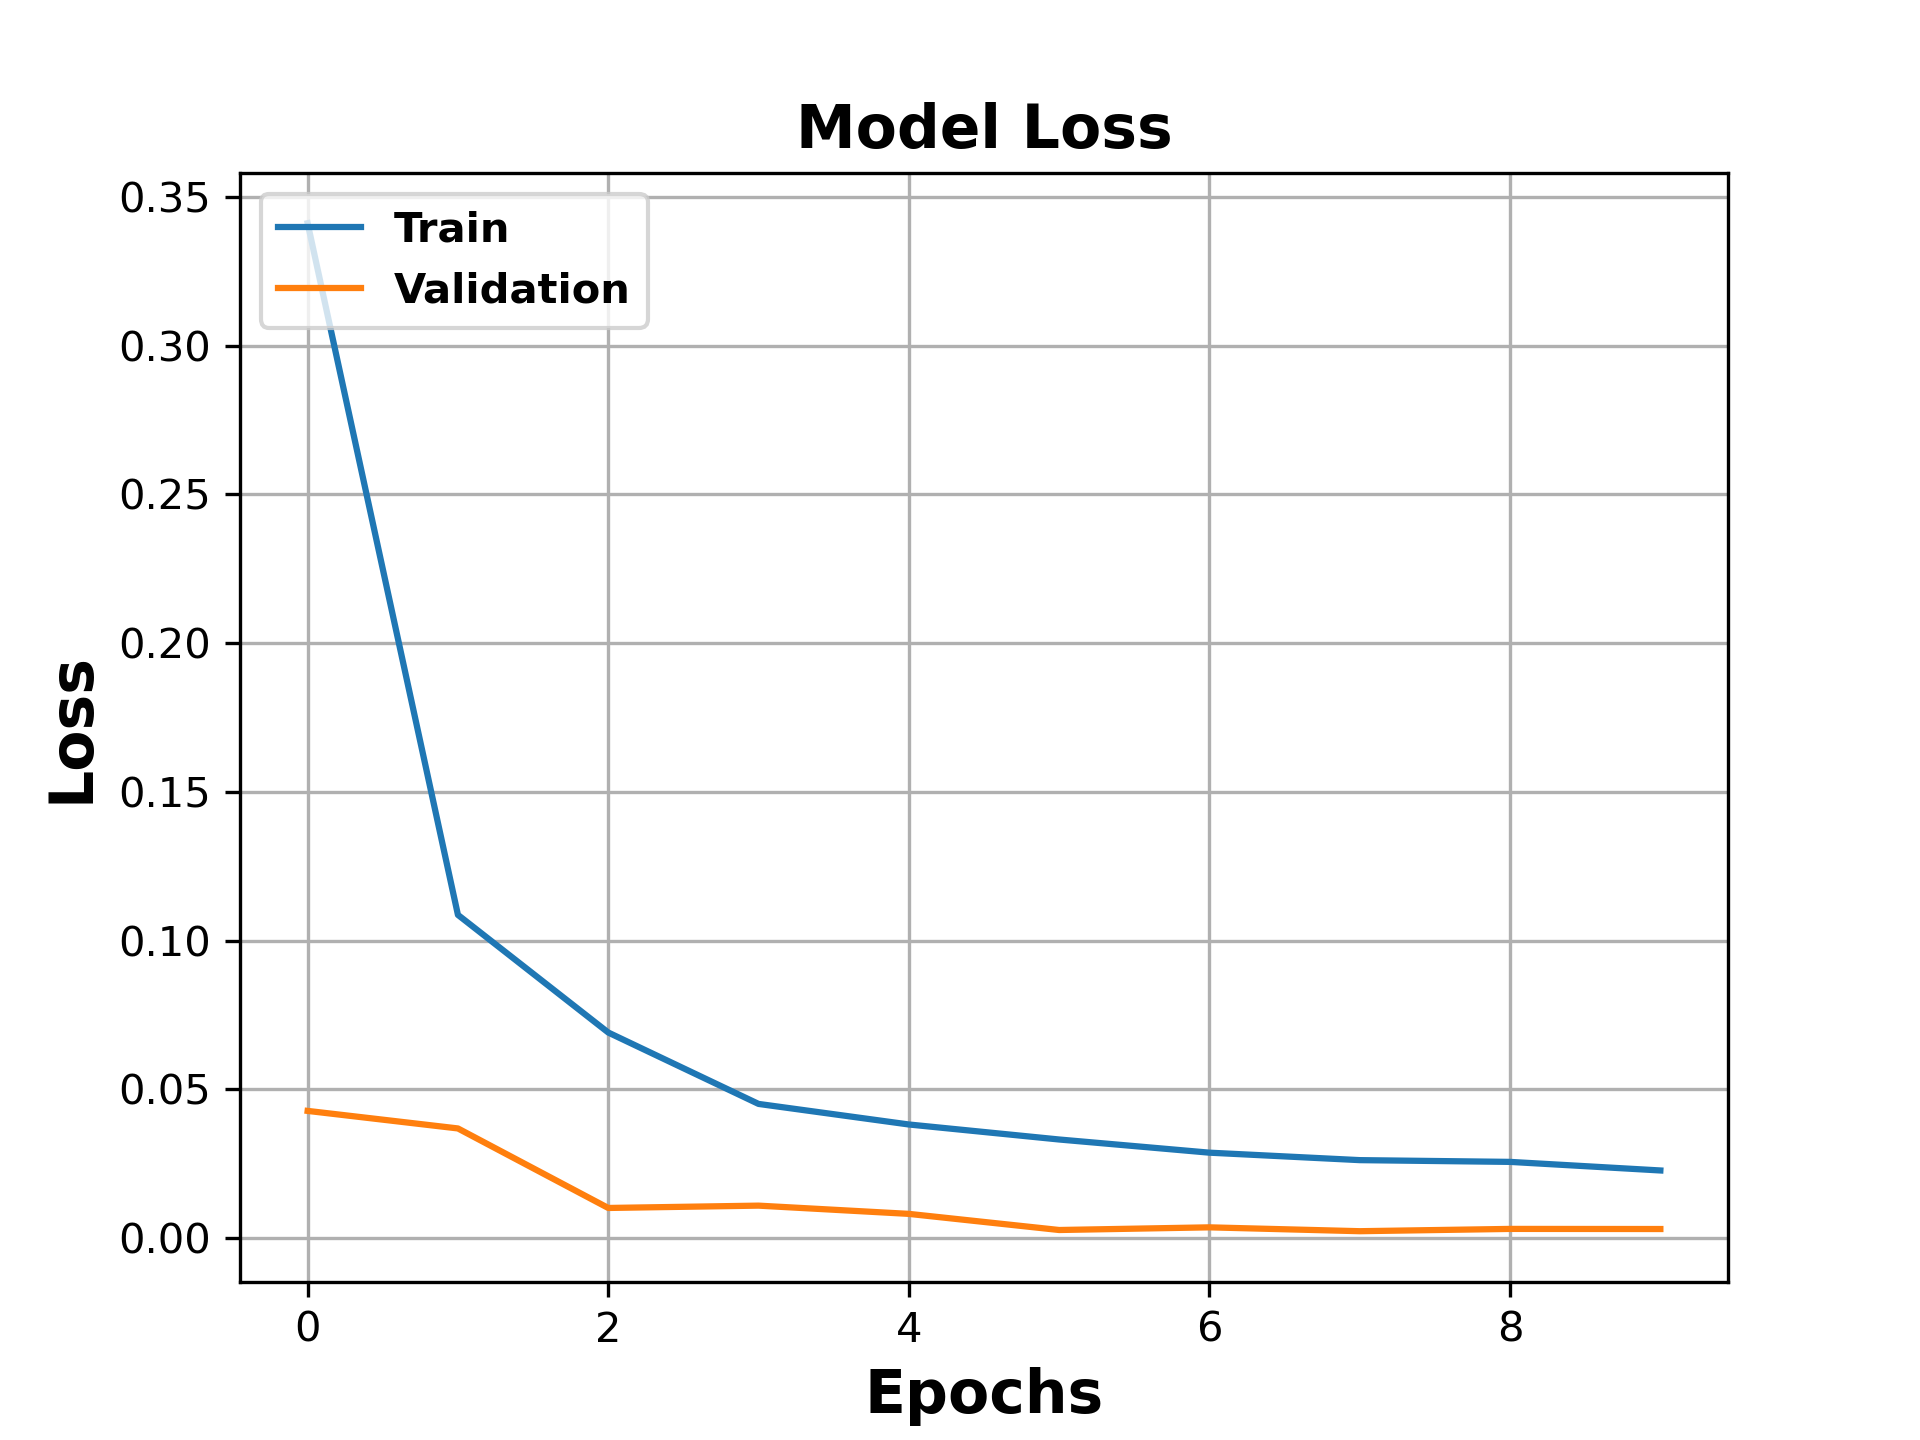
\includegraphics[width=\textwidth]{images/Evaluation/Faxified_Data_Classifier_2021-05-31_19-31-35_Loss.png}
    \caption[Epoch vs Loss Plot.]{Epoch vs Loss Plot.}
    \label{fig:FaxifiedClassifierLoss}
  \end{minipage}
\end{figure}



\begin{figure}[H]
        \begin{center}
	    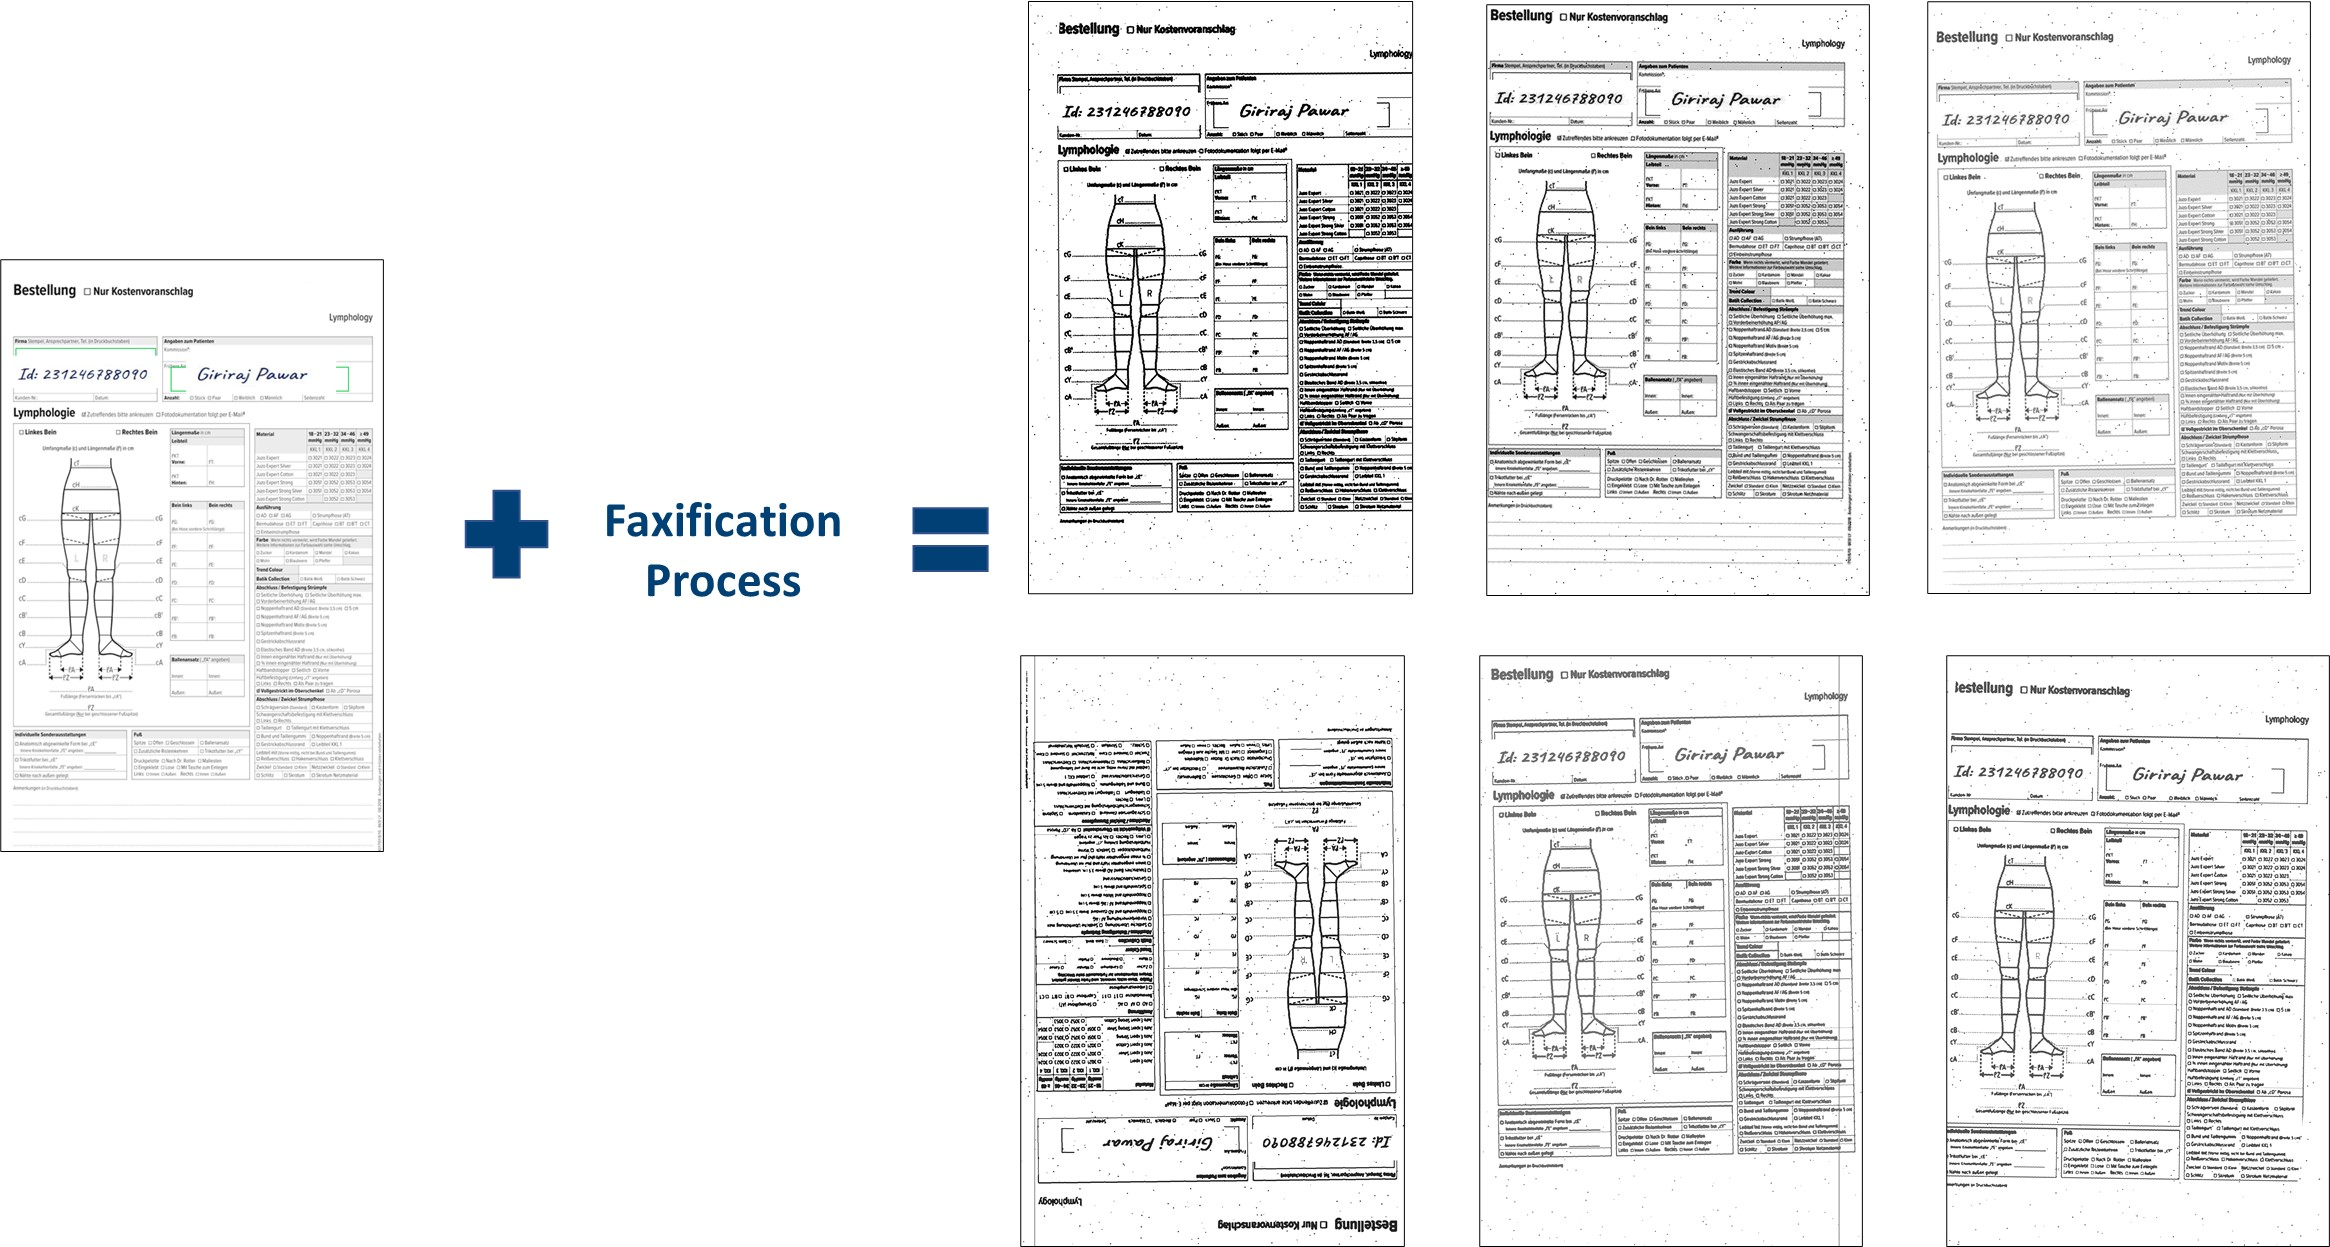
\includegraphics[scale=0.25]{images/Evaluation/FaxificationProcess.jpg}
	    \caption[Illustration of faxification process applied on synthetic document images.]{Illustration of faxification process applied on synthetic document images.}
	    \label{fig:FaxificationProcess}
	    \end{center}
\end{figure}



\begin{figure}[H]
        \begin{center}
	    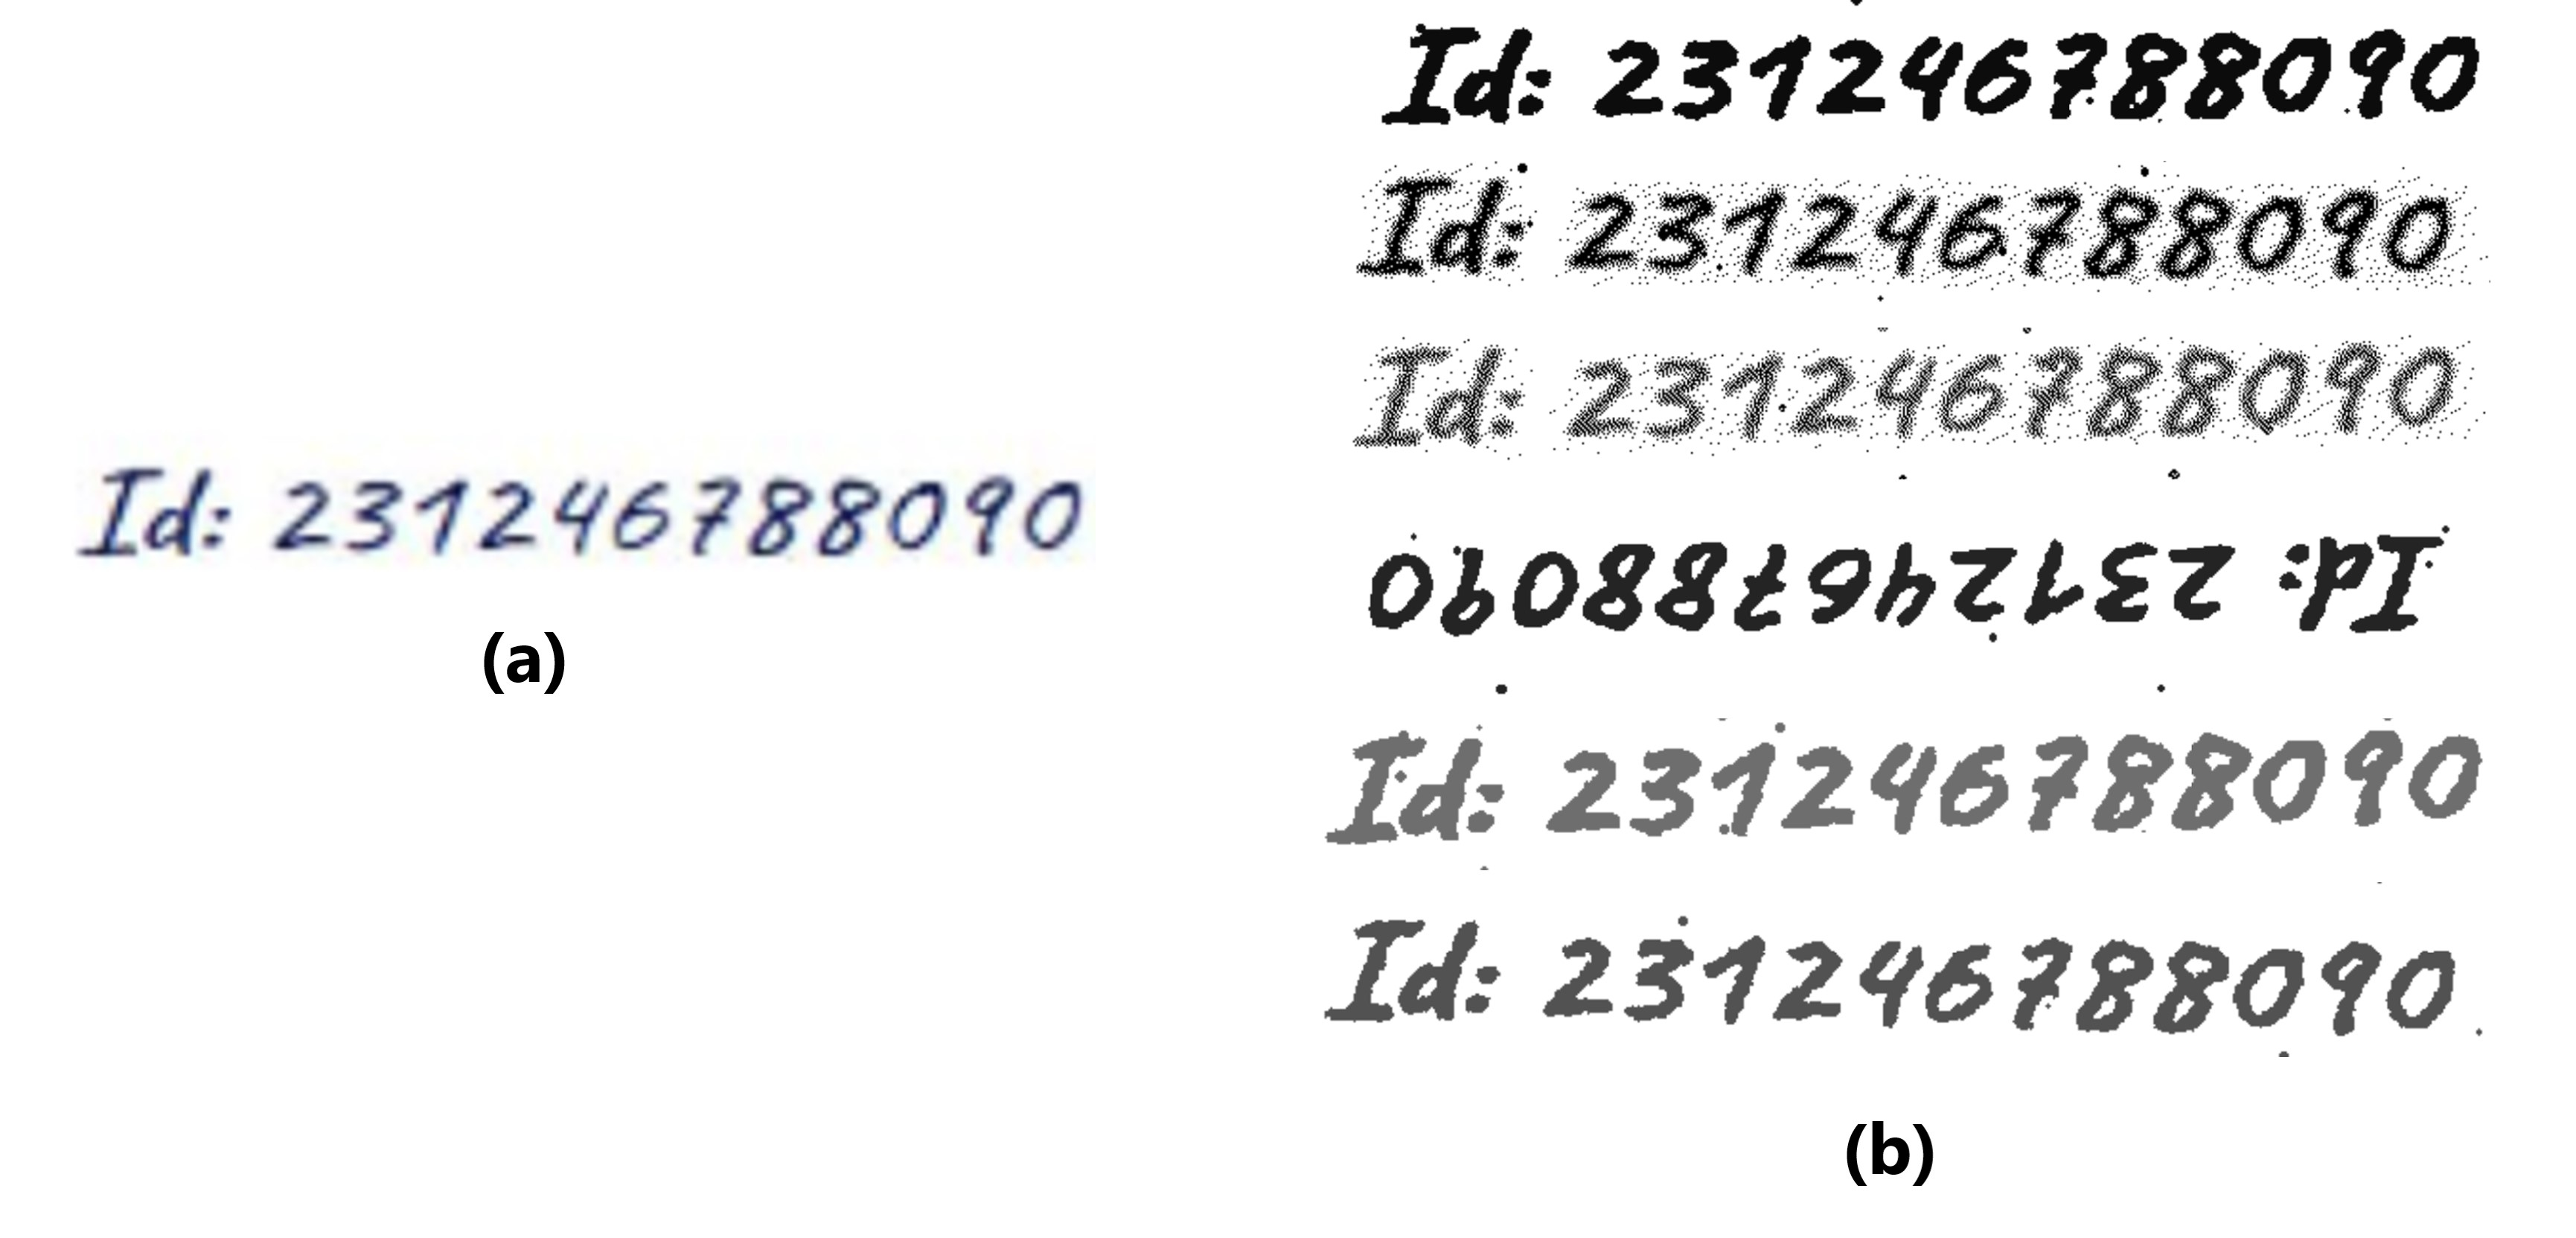
\includegraphics[scale=0.15]{images/Evaluation/FaxificationProcessZoomed.jpg}
	    \caption[Illustration of faxified document images to conclude that faxification process is a random process, the input images are faxified randomly to create distinct output.]{Illustration of faxified document images to conclude that faxification process is a random process, the input images are faxified randomly to create distinct and random output. For example, for a snippet in a synthetic document image (a), snippets of faxified document images shown in (b) are created distinct and random.}
	    \label{fig:FaxificationProcessZoomed}
	    \end{center}
\end{figure}






\begin{center}
\begin{table}[H]
    \begin{center}
    \begin{tabular}{P{0.22\linewidth} P{0.10\linewidth} P{0.10\linewidth} P{0.10\linewidth} P{0.10\linewidth}} 
        \toprule
            & Precision & Recall & F1-score & Support\\[0.0ex] 
        \midrule
        DE\_LY\_Arm\_2020-01 & 0.97 & 0.75 & 0.85 & 44\\[0.0ex]
        \midrule
        DE\_LY\_Bein\_2018-08 & 1.00 & 0.53 & 0.69 & 47\\[0.0ex]
        \midrule
        DE\_LY\_Bein\_2019-01 & 0.74 & 0.34 & 0.47 & 50\\[0.0ex]
        \midrule
        DE\_LY\_Bein\_2019-07 & 0.53 & 1.00 & 0.69 & 60\\[0.0ex]
        \midrule
        DE\_LY\_Bein\_2020-01 & 1.00 & 0.17 & 0.29 & 624\\[0.0ex]
        \midrule
        DE\_LY\_Bein\_2020-03 & 0.19 & 0.98 & 0.32 & 128\\[0.0ex]
        \midrule
        DE\_LY\_Hand\_2020-01 & 0.21 & 1.00 & 0.34 & 16\\[0.0ex]
        \midrule
        DE\_PH\_Bein\_2018-09 & 0.68 & 0.68 & 0.68 & 22\\[0.0ex]
        \midrule
        DE\_PH\_Bein\_2019-02 & 0.78 & 0.64 & 0.71 & 28\\[0.0ex]
        \midrule
        DE\_PH\_Bein\_2020-01 & 1.00 & 0.59 & 0.74 & 143\\[0.0ex]
        \midrule
        \midrule
        Accuracy              &      &      & \bf{0.43} & 1162\\[0.0ex]
        Macro average             & 0.71 & 0.67 & \bf{0.58} & 1162\\[0.0ex]
        Weighted average          & 0.85 & 0.43 & \bf{0.43} & 1162\\[0.0ex]

        \bottomrule
    \end{tabular}
    \caption[Classification report generated after the classifier is trained on faxified document images, its classification performance evaluated on the annotated real document images.]{Classification report generated after the classifier is trained on faxified document images, its classification performance evaluated on the annotated real document images.}
    \label{table:FaxifiedClassificationReport}
    \end{center}
\end{table}
\end{center}







\section{Results}\label{results}


\subsection{Qualitative Results}

The qualitative results look very promising. It is observed mode collapse has not occurred after training \ac{CycleGAN} for 20 epochs and with the dataset of 100,000 images in both domains and batch size 1. In Section \ref{FailureCases} failure cases like, no reconstrcution of handwritten crop in the target domain and unecessary noise.

\begin{figure}[H]
        \begin{center}
	    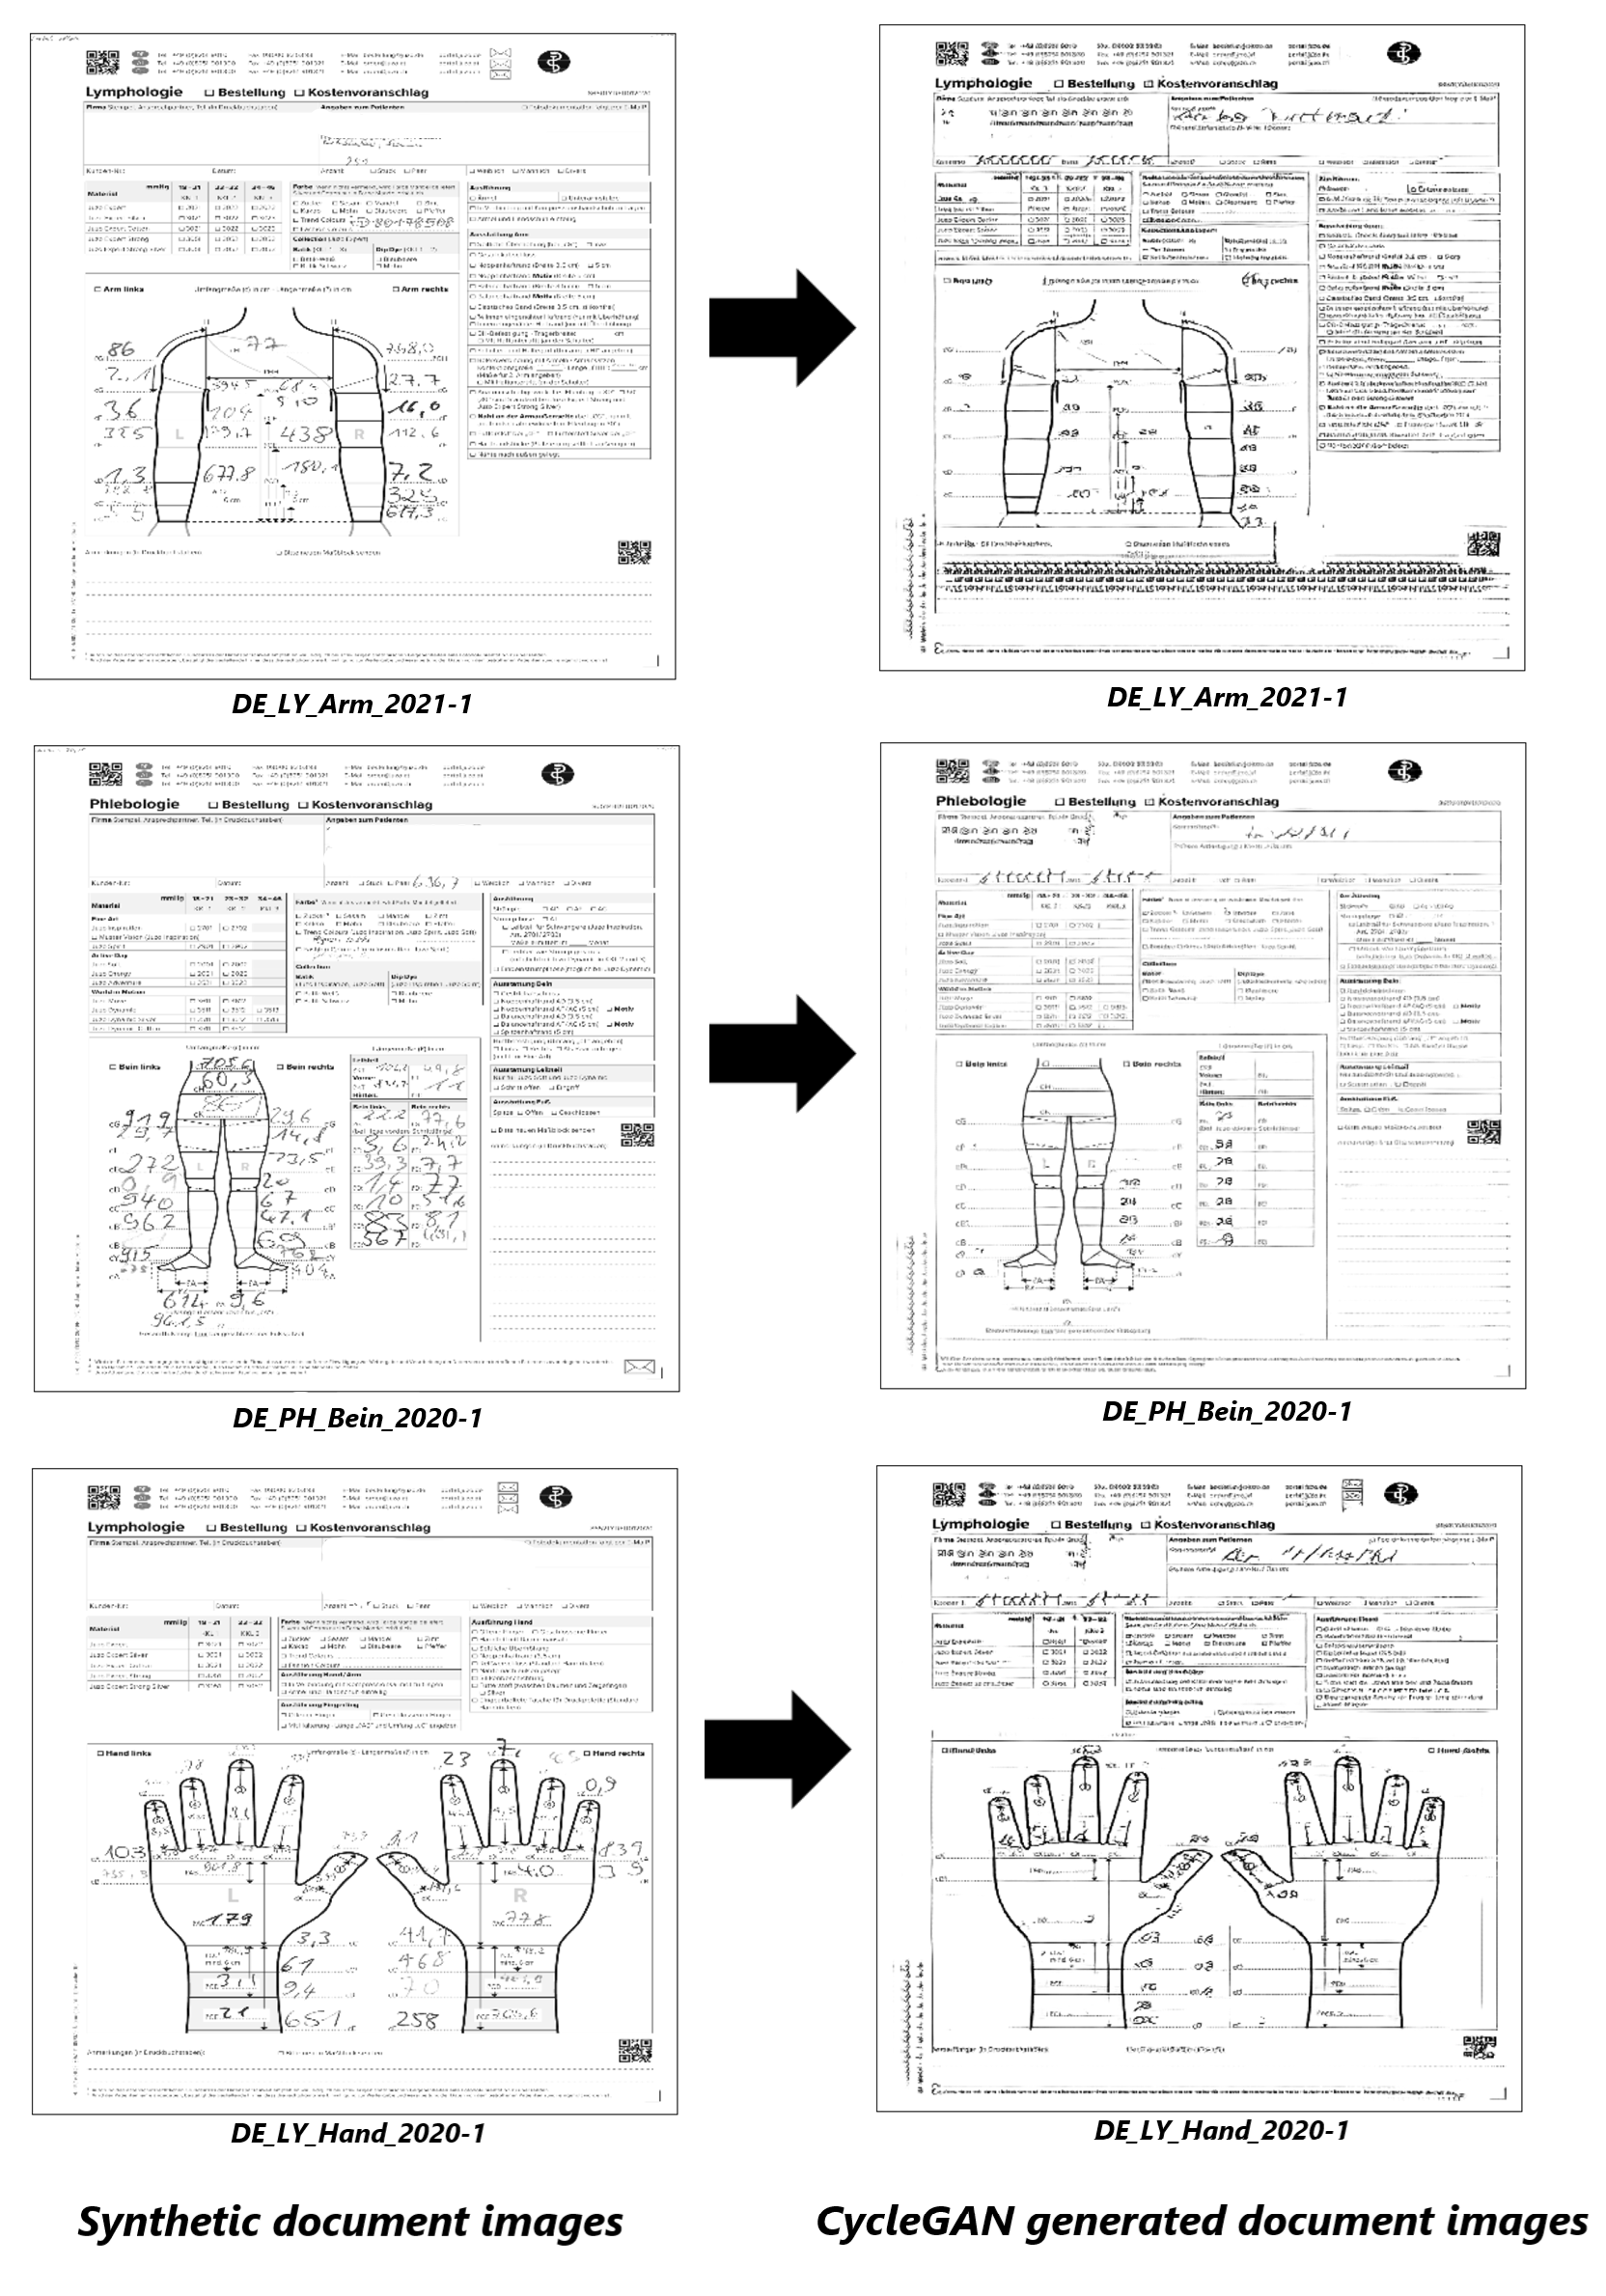
\includegraphics[scale=0.30]{images/Evaluation/Qualitative_Results.png}
	    \caption[Synthetic document images transformed into realistic document images by our image-to-image translation application implemented using \ac{CycleGAN}.]{Synthetic document images transformed into realistic document images by our image-to-image translation application implemented using \ac{CycleGAN}. The generator $G$ ($G: X \rightarrow Y$) in \ac{CycleGAN} model is used, to transform synthetic document image (from source domain) into realistic document image (in the target domain).}
	    \label{fig:QualitativeResults}
	    \end{center}
\end{figure}


\subsubsection{Failure Cases}\label{FailureCases}




\subsection{Quantitative Results}

\begin{center}
\begin{table}[H]
    \begin{center}
    \begin{tabular}{P{0.35\linewidth} P{0.12\linewidth} P{0.20\linewidth} P{0.20\linewidth}} 
        \toprule
        \bf{Classifier trained using} & \bf{Accuracy}  & \bf{Weighted average F1-score} & \bf{Macro average F1-score} \\[0.0ex] 
	 \midrule
        \bf{Synthetic document images} & 25\% & 31\% & 27\%\\[0.0ex]
        \midrule
       \bf{\ac{CycleGAN} generated document images} & 27\% & 25\% & 34\%\\[0.0ex]
        \midrule
        \bf{Faxified document images} & 43\% & 43\% & 58\%\\[0.0ex]
        \bottomrule
    \end{tabular}
    \caption[Comparison of accuracy and F1-scores when the classifiers trained on different data distributions and evaluated on annotated real document images.]{Comparison of accuracy and F1-scores when the classifiers trained on different data distributions and evaluated on annotated real document images.}
    \label{table:finalResults}
    \end{center}
\end{table}
\end{center}





\begin{figure}[H]
        \begin{center}
	    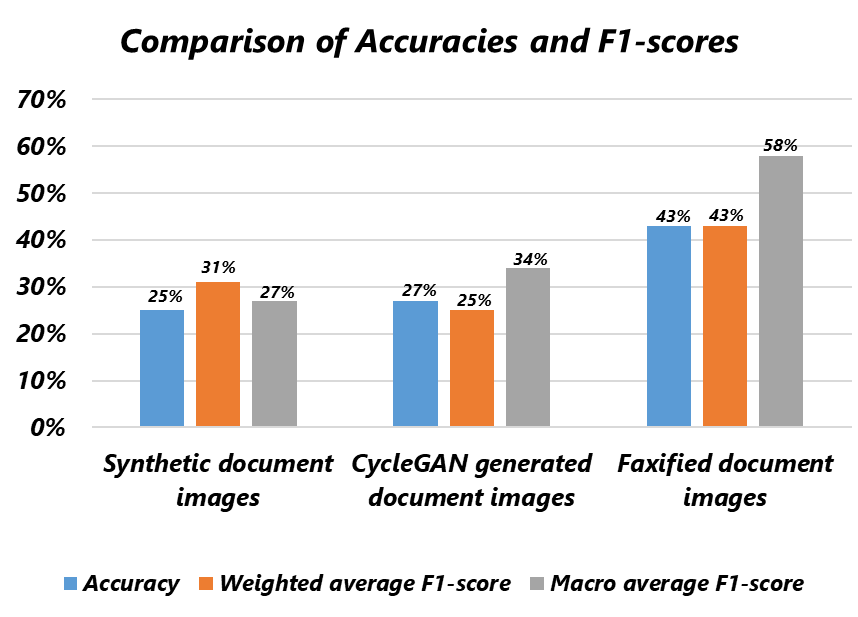
\includegraphics[scale=0.60]{images/Evaluation/ComparisonOfAccuracyAndF1Score.png}
	    \caption[Plot of accuracy and F1-scores when the classifiers trained on different data distributions and evaluated on annotated real document images.]{Plot of accuracy and F1-scores when the classifiers trained on different data distributions and evaluated on annotated real document images.}
	    \label{fig:ComparisonOfAccuracyAndF1Score}
	    \end{center}
\end{figure}
















%%%%%%%%%%%%%%%%%%%%%%%%%%%%%%%%%%%%%%%%%%%%%%%%%%%%%%%%%%%%%%%%%%%%%%%%%%%%%%%%%%%%%%%%%%%%%%%%%%%%%%%%%%%%%%%%%%%

%\subsection{Overview of Domain Gap between Distribution}
\begin{comment}
\begin{figure}[H]
        \begin{center}
	    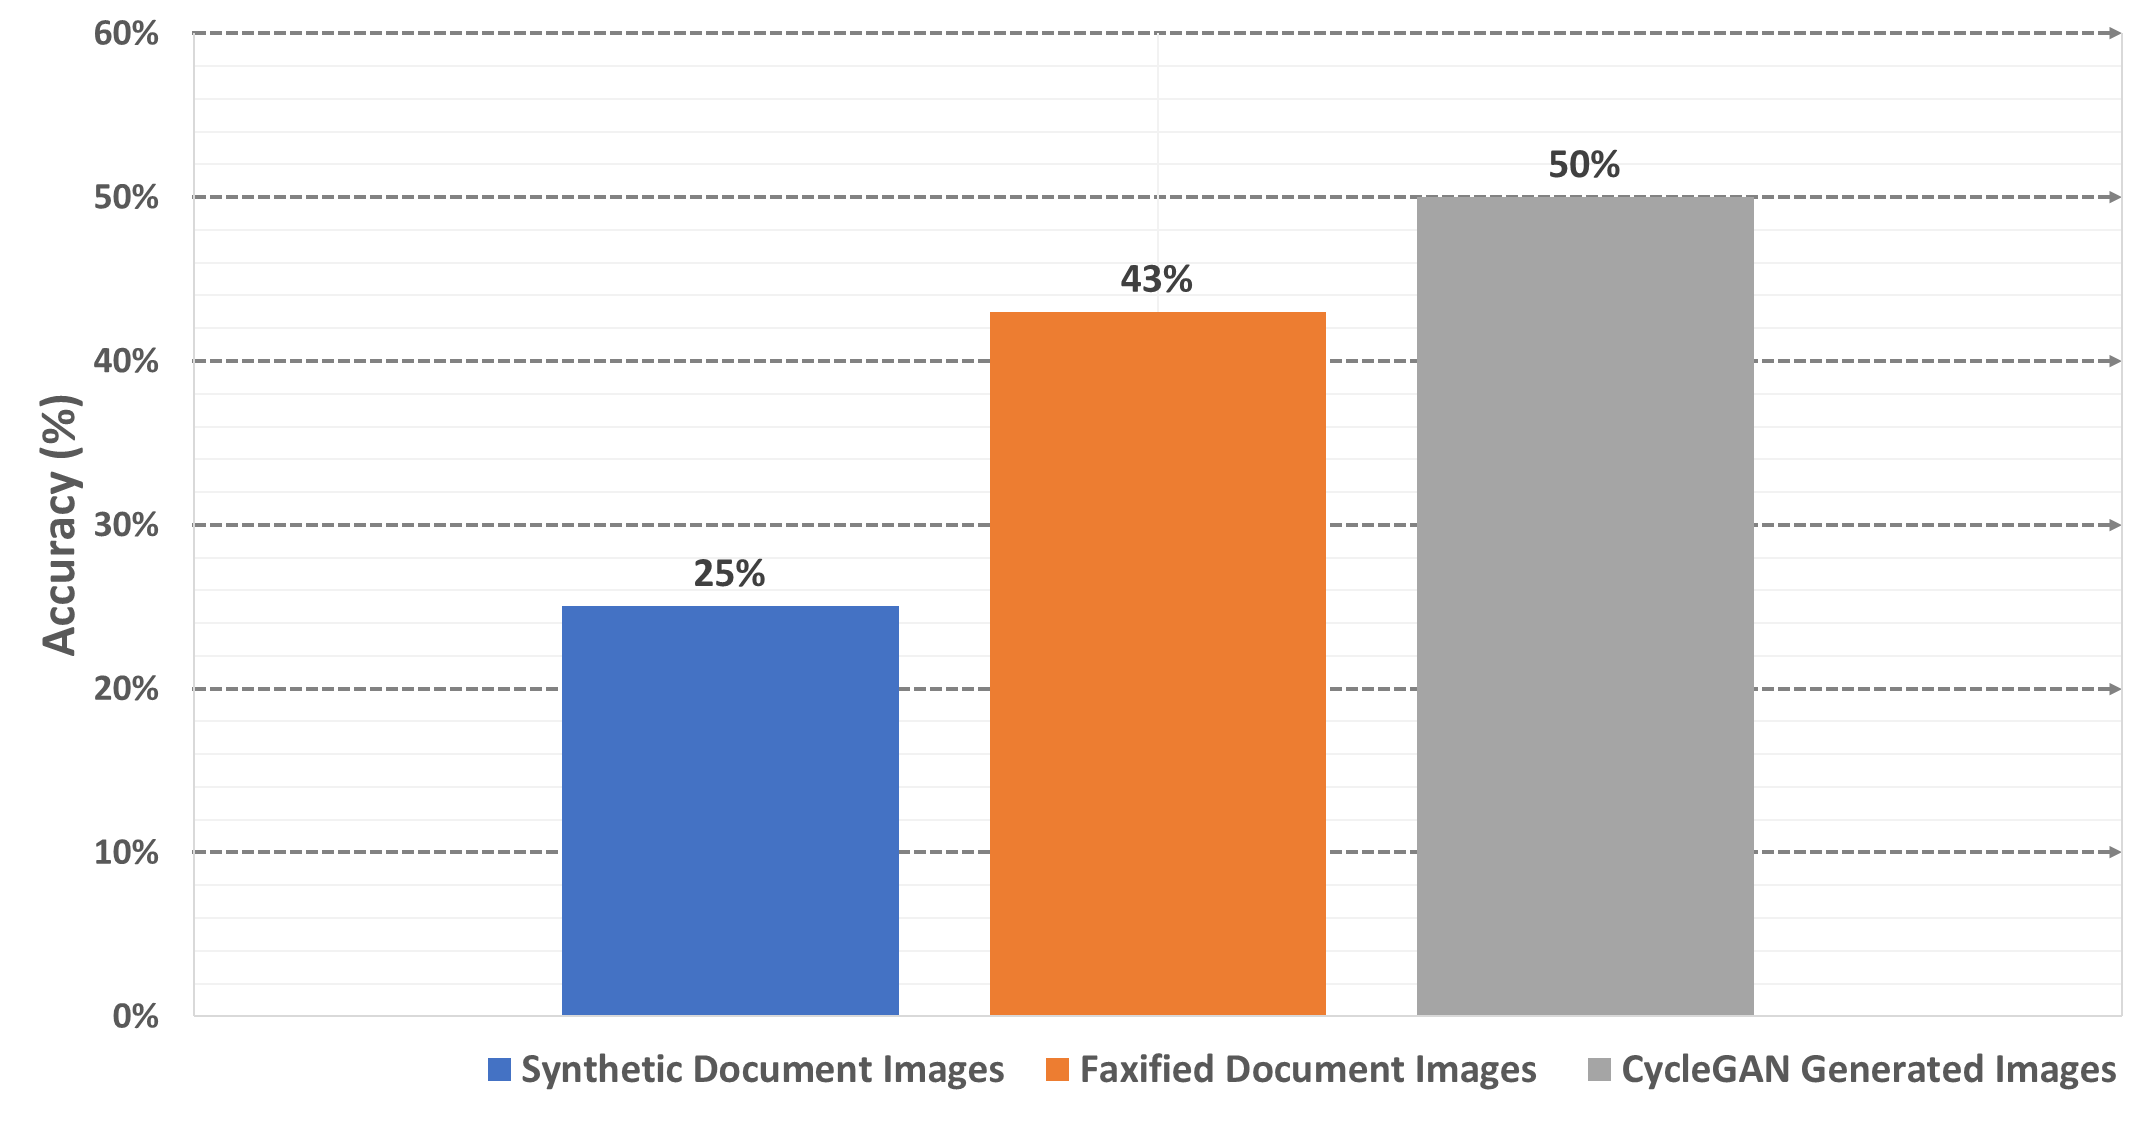
\includegraphics[scale=0.20]{images/DomainGap.png}
	    \caption[Illustration of Domain Gap Between Real Data Distribution and Synthetic Data Distribution, Faxified Data Distribution, and \ac{CycleGAN} Generated Data Distribution.]{Illustration of Domain Gap Between Real Data Distribution and Synthetic Data Distribution, Faxified Data Distribution, and \ac{CycleGAN} Generated Data Distribution. Initially, the classifiers are trained on Synthetic Document Images, Faxified Document Images, and \ac{CycleGAN} Generated Document Images. Later their Classification Performance Evaluated on the Annotated Real Document Images to understand the Domain Gap between distributions using Accuracy as an Evaluation Metric.}
	    \label{fig:DomainGap}
	    \end{center}
\end{figure}
\end{comment}

%To evaluate the quality of images generated by the \ac{CycleGAN}, a classifier is trained on the \ac{CycleGAN} generated data and its accuracy on a real dtest dataset is used as a metric to measure how well the \ac{CycleGAN} model distribution matches the real data distribution. Basically, The classification capability of the trained classifier is used as an objective measure to assess the quality of images generated by \ac{CycleGAN}. Also, the classifier is trained on the synthetic document images and it's accuracy evaluated in 
%Classification report and metrics
%Three separate classifiers are trained upon synthetic data distribution, faxified data distribution, and \ac{CycleGAN} generated data distribution respectively. After training the classifiers they have evaluated annotated real document images. Using this performance evaluation using metrics like weighted f1 score and accuracy 	


\begin{comment}
\begin{center}
\begin{table}[H]
    \begin{center}
    \begin{tabular}{P{0.30\linewidth} P{0.15\linewidth} P{0.20\linewidth} P{0.20\linewidth}} 
        \toprule
        \bf{Data Distributions} & \bf{Accuracy}  & \bf{Weighted average F1-score} & \bf{Macro average F1-score} \\[0.0ex] 
        \midrule
        \bf{Synthetic document images} & 25\% & 31\% & 27\%\\[0.0ex]
        \midrule
       \bf{\ac{CycleGAN} generated document images} & 27\% & 47\% &34\%\\[0.0ex]
        \midrule
        \bf{Faxified document images} & 43\% & 43\% & 58\%\\[0.0ex]
        \bottomrule
    \end{tabular}
    \caption[Comparison of accuracy and F1-scores when the classifiers trained on different data distributions and evaluated on annotated real document images.]{Comparison of accuracy and F1-scores when the classifiers trained on different data distributions and evaluated on annotated real document images.}
    \label{table:finalResults}
    \end{center}
\end{table}
\end{center}




\begin{center}
\begin{table}[H]
    \begin{center}
    \begin{tabular}{P{0.22\linewidth} P{0.22\linewidth} P{0.22\linewidth} P{0.22\linewidth}} 
        \toprule
        \bf{Classifier trained using} & \bf{Accuracy on annotated real document images}  & \bf{Weighted average F1-score on annotated real document images} & \bf{Macro average F1-score on annotated real document images} \\[0.0ex] 
        \midrule
        \bf{Synthetic document images} & 25\% & 31\% & 27\%\\[0.0ex]
        \midrule
       \bf{\ac{CycleGAN} generated document images} & 27\% & 47\% &34\%\\[0.0ex]
        \midrule
        \bf{Faxified document images} & 43\% & 43\% & 58\%\\[0.0ex]
        \bottomrule
    \end{tabular}
    \caption[Comparison of accuracy and F1-scores when the classifiers trained on different data distributions and evaluated on annotated real document images.]{Comparison of accuracy and F1-scores when the classifiers trained on different data distributions and evaluated on annotated real document images.}
    \label{table:finalResults}
    \end{center}
\end{table}
\end{center}

\end{comment}